\documentclass[10pt,a4paper]{article}
\usepackage[top=2.54cm,bottom=2.54cm,left=2.54cm,right=2.54cm]{geometry}
\usepackage[utf8]{inputenc} 
\usepackage[T1]{fontenc}   
\usepackage{indentfirst}
\setlength{\parindent}{2em}
\usepackage{multicol}
\usepackage{setspace}
\usepackage{bm}
\usepackage{pifont}
\usepackage{float}
\usepackage{amssymb}
\usepackage[tbtags]{amsmath} 
\usepackage{tikz}
\usepackage{subcaption}

\usetikzlibrary{arrows.meta}
\tikzset{
    dot/.style={circle, fill, inner sep=1.5pt}, % 定义格点的样式
    main plot/.style={scale=0.7, font=\small} % 定义每个子图的通用样式
}

\usepackage[
    backend=biber,      
    style=numeric-comp, 
    sorting=none        
]{biblatex}
\addbibresource{references.bib} 
\usepackage{hyperref}

\numberwithin{equation}{section}
\renewcommand{\baselinestretch}{1.5}

\newcommand{\ket}[1]{\left| #1 \right\rangle}
\newcommand{\vev}[1]{\left\langle #1 \right\rangle}

\newcommand{\TheTitle}{Fusion products of representations of the $\widehat{\mathfrak{sl}_{2}}$ algebra}
\newcommand{\StudentName}{Hexuan Li}
\newcommand{\StudentAffiliation}{École Polytechnique, ETH Zürich} % Can add more lines with \\

\newcommand{\SupervisorName}{Sylvain Ribault}
\newcommand{\SupervisorAffiliation}{IPhT, CEA Saclay}

% The \today command automatically inserts the current date. 
% You can also set it manually, e.g., \newcommand{\TheDate}{July 7, 2025}
\newcommand{\TheDate}{\today} 

\begin{document}

\thispagestyle{empty}

% The entire title block is centered.
\begin{center}

    % --- TITLE ---
    {\LARGE\bfseries \TheTitle \par}

    \vspace{2cm} % Adjust space as needed

    % --- AUTHOR ---
    {\large \StudentName \par}
    {\itshape \StudentAffiliation \par}

    \vspace{1.5cm} % Adjust space as needed

    % --- ADVISOR ---
    Advisor: {\large \SupervisorName \par}
    {\itshape \SupervisorAffiliation \par}
    
    \vspace{1.5cm} % Adjust space as needed
    
    % --- DATE ---
    (Dated: \today)

\end{center}

\vspace{2cm} % Space between the title block and the main text

% --- INTRODUCTORY TEXT / ABSTRACT ---
% This text is outside the \center environment to be left-aligned and justified.
% \noindent prevents the first line from being indented.
\noindent
\textbf{ABSTRACT}: In this thesis, we review the representations that appear in the $\widetilde{SL}_{2}(\mathbb{R})$ WZW model and the degenerate representations that are needed 
    to bootstrap this model. 
    We determine fusion rules of level 1 degenerate representations with affine highest weight representations by 
    solving null vector equations in both spectral flow preserving and violating cases. 

% This second \vfill pushes the content block up from the bottom,
% perfectly centering it on the page between the top and bottom margins.
\newpage

\tableofcontents

\section{Introduction and overview}
The $\widetilde{SL}_{2}(\mathbb{R})$ Wess-Zumino-Witten (WZW) model is a conformal field theory (CFT) with an 
$\widehat{\mathfrak{sl}_{2}}$ symmetry. The study of the $\widetilde{SL}_{2}(\mathbb{R})$ WZW model is motivated by 
its connection with string theory in $AdS_{3}$. The fusion rules of WZW models at fractional level have been well studied, 
where there exist doubly degenerate representations. One set of the fusion rules of these models has been proposed by 
Awata and Yamada \cite{Awata:1992sm}. However, this model at generic level has not been completely solved: the 3-point function is not 
fully known and crossing symmetry has not been proved yet. 

One important feature of the $\widetilde{SL}_{2}(\mathbb{R})$ WZW model is the spectral flow. Maldacena and Ooguri have shown that the 
physical spectrum cannot be built only from affine primaries but should also include spectral flowed fields \cite{Maldacena:2001km}. 
They proposed a well-tested and widely believed spectrum of this model as well as the fusion rules.

In order to solve this model, one needs to find the null vectors and the fusion rules between degenerate representations and other 
representations, as was done in solving the Liouville theory \cite{Ribault:2014hia} and the $H^{+}_{3}$-WZNW model \cite{Teschner:1997ft}. 
One null vector of the $\widetilde{SL}_{2}(\mathbb{R})$ WZW model was given in \cite{Stocco:2022gah}. 
However, only the spectral flow preserving fusion rules are considered in \cite{Stocco:2022gah}. Hence the deduced 
fusion rules are incomplete. 

In this thesis, we initiate the study of some spectrally flowed degenerate representations. We find that the action of spectral flow on a 
degenerate representation might give another degenerate representation at higher level. We determine fusion rules between degenerate 
representations and generic representations as shown in \eqref{mainresult}, by solving the null vector equations. 
We find the fusion with degenerate representations will also give spectral flowed representations. 

This thesis is organized as follows. We give a brief review of the $\widetilde{SL}_{2}(\mathbb{R})$ model in section 2. In section 3, we 
introduce the degenerate representations and give the spectrum of the level 1 degenerate representations. In section 4, we apply the null 
vector to the three-point functions to calculate the fusion rules between degenerate representations and affine highest-weight representations.

\section{\texorpdfstring{$\widetilde{SL}_{2}(\mathbb{R})$}{Lg} WZW model}
In this chapter, we introduce the theoretical foundation of the WZW model, especially concentrating on the 
$\widetilde{SL}_{2}(\mathbb{R})$ case. We begin by defining the non-Abelian affine symmetries and introducing the Sugawara construction. 
Then, we define fields and representations that appear in this model. 
At last, we give the correlation functions that are necessary to solve this model. 

\subsection{Non-Abelian affine symmetries}
\subsubsection*{Reminders on Lie algebras}
A Lie algebra is a vector space $\mathfrak{g}$ equipped with a binary operation $\left[\cdot,\cdot \right]:\mathfrak{g}\times \mathfrak{g} \rightarrow \mathfrak{g}$,
known as the Lie bracket, which satisfies the following axioms:
\begin{itemize}
    \item Bilinearity:$\quad \left[ax+by,z \right] = a \left[x,z\right] + b \left[y,z\right],\quad \left[z,ax+by \right] = a \left[z,x\right] + b \left[z,y\right]$.
    \item Antisymmetry:$\quad \left[x,y\right] = - \left[y,x\right]$.
    \item Jacobi identity:$\quad \left[a,\left[b,c\right]\right]+\left[b,\left[c,a\right]\right]+\left[c,\left[a,b\right]\right] = 0$.
\end{itemize}
For a basis of generators $t^{a}$ of $\mathfrak{g}$, the Lie bracket is defined by the commutation relations:
\begin{equation}
    \left[t^{a},t^{b}\right] = f^{ab}_{c} t^{c}.
\end{equation}
The numbers $f^{ab}_{c}$ are called structure constants of the Lie algebra. From these, one can define an invariant symmetric tensor 
called the Killing tensor: 
\begin{equation}
    K^{ab} = \frac{1}{2g} f^{ac}_{d}f^{bd}_{c},
\end{equation}
where $g$ is the dual Coxeter number of $\mathfrak{g}$. For the case of $\mathfrak{sl}_{2}$, this number is $g = 2$. The non-zero 
coefficients are:
\begin{equation}
    K^{00} = \frac{1}{2}, \quad K^{+-} = K^{-+} = 1.
\end{equation}

We define the quadratic Casimir operator $C$ as 
\begin{equation}
    C = K_{ab} t^{a} t^{b}.
\end{equation}
$C$ is a central element of the universal enveloping algebra $U(\mathfrak{g})$, which means that 
$C$ commutes with all Lie algebra generators: $\left[C,t^{a}\right] = 0$. This implies that in an irreducible representation, 
the Casimir operator is proportional to the identity. 

For the algebra $\mathfrak{sl}_{2}$, the irreducible representations are labeled by a number $j$, called the spin. 
The eigenvalue of the Casimir operator is 
\begin{equation}
    C = 2 t^{0} t^{0} + t^{+} t^{-} + t^{-} t^{+} = 2j(j+1).
\end{equation}

\subsubsection*{Symmetry algebra}
We now define the symmetry algebra of the WZW model. 
The $G$ WZW model is a CFT with an infinite-dimensional affine Lie algebra, denoted as $\hat{\mathfrak{g}}_{k}$. 
This algebra is generated by dim$\mathfrak{g}$ holomorphic currents $J^{a}(z)$ through their operator product expansions(OPEs), 
\begin{equation}
    \boxed{
        J^{a}(z)J^{b}(w) = \frac{kK^{ab}}{(z-w)^{2}} + \frac{f^{ab}_{c} J^{c}(w)}{z-w} + \mathcal{O}(1), \label{OPEJJ}
        }
\end{equation}
where the constant $k$ is the level, which is the most important parameter of the model. 

The modes of the current are defined by 
\begin{equation}
    J^{a}_{n} = \oint \mathrm{d}z \, z^{n} J^{a}(z).
\end{equation}
From the OPEs \eqref{OPEJJ}, we deduce the following commutation relations, 
which formally define the affine Lie algebra $\widehat{\mathfrak{sl}}(2)_{k}$
\begin{equation}
    \boxed{
        \left[ J^{a}_{m}, J^{b}_{n} \right] = f^{ab}_{c} J^{c}_{m+n} + m k K^{ab} \delta_{m+n,0}. \label{CR1}
    }
\end{equation}

\subsubsection*{The Sugawara construction}
The symmetry algebra of 2D CFT is the Virasoro algebra. The generators of the Virasoro algebra are $\left(L_{n}\right)_{n \in \mathbb{Z}}$, and 
the commutation relations are 
\begin{equation}
    \boxed{
        \left[L_{m},L_{n}\right] = (m-n)L_{m+n} + \frac{c}{12} (n-1)n(n+1) \delta_{n+m,0}.
    }
\end{equation}
We define a holomorphic field $T(y)$ as a generating function for $\left(L_{n}\right)$, known as the energy-momentum tensor:
\begin{equation}
    T(y) = \sum_{n\in \mathbb{Z}} \frac{L_{n}^{(z)}}{(y-z)^{n+2}},
\end{equation}
where $L_{n}^{(z)}$ is the Virasoro generator at $z$. The OPE between $T$ and itself is 
\begin{equation}
    T(y) T(z) = \frac{c/2}{(y-z)^{4}} + \frac{2 T(z)}{(y-z)^{2}} + \frac{\partial_{z} T(z)}{y-z} + \mathcal{O}(1).
\end{equation}
A Virasoro primary field $V_{\Delta}(z)$ with conformal dimension $\Delta$ is defined by its OPE with $T(y)$: 
\begin{equation}
    T(y) V_{\Delta}(z) = \frac{\Delta V_{\Delta}(z)}{(y-z)^{2}} + \frac{\partial_{z} V_{\Delta}(z)}{y-z} + \mathcal{O}(1).
\end{equation}

In the WZW model, we introduce the Sugawara construction for the energy momentum tensor $T(z)$: 
\begin{equation}
    \boxed{
        T(z) = \frac{K_{ab}}{2(k-g)} : J^{a}(z) J^{b}(z) : . \label{EM}
        } 
\end{equation}
The central charge of $T(z)$ is $c = \frac{k \mathrm{dim} \mathfrak{g}}{k-g}$. In our case of $\widetilde{SL}_{2}(\mathbb{R})$ 
WZW model, this gives 
\begin{equation}
    \boxed{
        c = \frac{3k}{k-2}
        }
\end{equation}

The Virasoro generators are given by
\begin{equation}
    L_{n} = \frac{K_{ab}}{2(k+g)} : \sum_{m \in \mathbb{Z} } J^{a}_{n-m} J^{b}_{m} :. \label{DefLn}
\end{equation}
Using the commutation relations for the $J^{a}_{n}$ \eqref{CR1}, we can deduce commutation relation between $L_{m}$ and $J^{a}_{n}$:
\begin{equation}
    \boxed{
            \left[ L_{m}, J^{a}_{n} \right] = -n J^{a}_{m+n}. \label{CR2}
    }
\end{equation}

\subsection{Affine primary fields}
An affine primary field $\phi^{j}(z)$ associated with representation $\mathcal{R}^{j}$ is defined by its OPE with the current field 
$J^{a}(y)$:
\begin{equation}
    \boxed{
        J^{a}(y) \phi^{j}(z) \sim \frac{-(t^{a})^{T} \phi^{j}(z)}{y-z} + \mathcal{O}(1), \label{OPEJPhi}
    }
\end{equation}
where $t^{a}$ is the generator of Lie algebra $\mathfrak{sl}_{2}$. This OPE involves the transposition of Lie algebra generators, which 
ensures the associativity of the OPE $J^{a}J^{b} \phi$. Since the transposition flips the sign of commutation relations, we need an additional 
minus sign.

The OPE between $T(y)$ and $\phi^{j}(z)$ can be obtained from the Sugawara construction \eqref{EM}:
\begin{equation}
    T(y) \phi^{j}(z) = \frac{K_{ab} t^{a}}{k-g} \left( \frac{\frac{1}{2} t^{b} \phi^{j}(z)}{(y-z)^{2}} - \frac{\left(J^{b} \phi^{j}\right)(z)}{y-z} \right) + \mathcal{O}(1).
\end{equation}
Hence an affine primary field is also a Virasoro primary field. 
The conformal dimension of $\phi^{j}(x)$ is proportional to the Casimir operator $C = K_{ab} t^{a} t^{b}$ :
\begin{equation}
    \boxed{
        \Delta_{j} = \frac{C(j)}{2(k-g)} = \frac{j(j+1)}{k-g}.
    }
\end{equation}

Based on the state-field correspondence, the field $\phi^{j}(z)$ corresponds to an affine primary state $\ket{v^{j}}$. 
The OPE \eqref{OPEJPhi} implies the action of current modes on this state:
\begin{equation}
    \left\{
        \begin{aligned}
            J^{a}_{n>0} \ket{v^{j}} &= 0,\\
            J^{a}_{0} \ket{v^{j}} &= - t^{a} \ket{v^{j}}.
        \end{aligned}
    \right.
\end{equation}

\subsubsection*{Isospin variables}
For practical calculations, especially for solving Ward identities, it is useful to realize the abstract action of the generators 
$t^{a}$ as differential operators acting on functions. We introduce the isospin variables and 
represent the fields as functions of the isospin variables, 
where $t^{a}$ act on primary fields as differential operators $D^{j}(t^{a})$. We introduce three important bases:

$x$-basis: In this basis, a field is represented as a function $\phi^{j}_{x}$, and $t^{a}$ acts as 
\begin{equation}
    \left\{
        \begin{aligned}
            D^{j}_{x}(t^{+}) &= x^{2} \partial_{x} - 2 j x, \\
            D^{j}_{x}(t^{0}) &= x \partial_{x} - j, \\
            D^{j}_{x}(t^{-}) &= - \partial_{x}.
        \end{aligned}
    \right. \label{Diffx}
\end{equation}
Because of the transposition in \eqref{OPEJPhi}, in the isospin formalism the generator $J^{a}_{0}$ acts as 
\begin{equation}
    J^{a}_{0} J^{b}_{0} \phi^{j}_{x}(z) = \left( -D^{j}_{x}\left(t^{b}\right) \right) \left( -D^{j}_{x}\left(t^{a}\right) \right) \phi^{j}_{x}(z).
\end{equation}

$\mu$-basis: The $t^{a}$ acts as 
\begin{equation}
    \left\{
        \begin{aligned}
            D^{j}_{x}(t^{+}) &= \mu \partial_{\mu}^{2} - \frac{j(j+1)}{\mu}, \\
            D^{j}_{x}(t^{0}) &= -\mu \partial_{\mu}, \\
            D^{j}_{x}(t^{-}) &= -\mu.
        \end{aligned}
    \right. \label{Diffmu}
\end{equation}

The $x$-basis field $\phi^{j}_{x}(z)$ and $\mu$-basis field $\phi^{j}_{\mu}(z)$ are related by the Fourier transform: 
\begin{equation}
    \phi^{j}_{x}(z) \sim \int \mathrm{d} \mu \, \mu^{-j-1} \mathrm{e}^{\mu x} \phi^{j}_{\mu}(z).
\end{equation}

$m$-basis: In this basis, the quadratic Casimir operator $C$ and $J^{0}_{0}$ are diagonalized. We denote the 
state in the $m$-basis to be $\ket{j,m}$. The action of 
$J^{\pm}_{0}$ on $\ket{j,m}$ is defined to be:
\begin{equation}
    \begin{aligned}
        J^{-}_{0} \ket{j,m} &= (j+m)\ket{j,m-1}, \\
        J^{0}_{0} \ket{j,m} &= m \ket{j,m} \\
        J^{+}_{0} \ket{j,m} &= (j-m)\ket{j,m+1}. \label{Jpm}
    \end{aligned}
\end{equation}
The field $\phi^{j}_{m}(z)$ corresponding to the state $\ket{j,m}$ is related to the $\mu$-basis field by 
\begin{equation}
    \phi^{j}_{m}(z) \sim \int \mathrm{d} \mu \, \mu^{-m} \phi^{j}_{\mu}(z).
\end{equation}


\subsection{Irreducible representations}
\subsubsection*{Irreducible representations of \texorpdfstring{$\mathfrak{sl}_{2}$}{Lg}}
For a given affine Lie algebra $\widehat{\mathfrak{g}}$, we define the horizontal algebra to be the subalgebra generated by zero-mode 
generators $J^{a}_{0}$. The central extension in \eqref{CR1} vanishes for $m = 0$, hence the subalgebra is isomorphic to the underlying 
Lie algebra $\mathfrak{g}$.

We work in the $m$-basis. From \eqref{Jpm}, we find two null states $J^{\pm}_{0}\ket{j,\pm}$, which satisfy the following vanishing 
condition:
\begin{equation}
    J^{\mp}_{0}\left(J^{\pm}_{0} \ket{j,\pm j}\right) = 0.
\end{equation}
Hence we can classify different representations by the existence of these states.

The representations appear in the spectrum can be classified into several series:
\begin{itemize}
    \item Principal continuous series $\mathcal{C}^{j}_{\alpha}$. They are labeled by spin $j \in -\frac{1}{2} + \mathrm{i} \mathbb{R}$ and 
    a real number $\alpha \in \left(0,1\right)$. The eigenvalue $m$ of $J^{0}_{0}$ is unbounded both above and below, taking values $m \in \alpha + \mathbb{Z}$.
    \item Discrete series $\mathcal{D}^{j,\pm}$. They are labeled by real spin $j \in (-\infty,\infty)$ and contain the state 
    $\ket{j,\mp j}$ respectively. Hence the spectrum is either bounded from below or from above.
\end{itemize}
Since $j$ and $-j-1$ correspond to the same quadratic Casimir operator, the representations with $j$ and $-j-1$ are equivalent. Hence 
only half of these representations are independent. 

Another crucial class of representations are the finite dimensional representations $\mathcal{E}^{j}$, which contain 
both $\ket{j,j}$ and $\ket{j,-j}$. They exist only 
when $j$ takes integer or half-integer values $j \in \mathbb{N}/2$, where $m$ takes values in $\{-j, -j+\frac{1}{2},\cdots,j-\frac{1}{2},j \}$.
We summarize the properties of these representations in the following table.
\begin{center}
    \begin{tabular}{|l|l|l|l|}
        \hline
        Representations&Parameter values&Eigenvalues of $J^{0}_{0}$&Conjugate representation\\
        \hline
        $\mathcal{C}^{j}_{\alpha}$ & $j \in -\frac{1}{2} + i \mathbb{R}_{+} $, $\alpha \in \mathbb{R}$ mod $\mathbb{Z}$& $\alpha + \mathbb{Z}$&$\mathcal{C}^{j}_{-\alpha}$\\
        $\mathcal{D}^{j,+}$ & $j \in (-\infty,-\frac{1}{2}) $& $-j + \mathbb{N}$&$\mathcal{D}^{j,-}$\\
        $\mathcal{D}^{j,-}$ & $j \in (-\infty,-\frac{1}{2}) $& $j - \mathbb{N}$&$\mathcal{D}^{j,+}$\\
        $\mathcal{E}^{j}$ & $j \in \mathbb{N}/2 $ & $\left\{-j,-j+\frac{1}{2}, \cdots, j-\frac{1}{2},j \right\}$&$\mathcal{E}^{j}$\\
        \hline
    \end{tabular}
\end{center}

The spectra of irreducible representations of $\mathfrak{sl}_{2}$ are plotted in figure \ref{fig:sl2}.
\begin{figure}[htbp!]
    \centering 
    \begin{subfigure}[b]{0.9\textwidth}
        \centering
        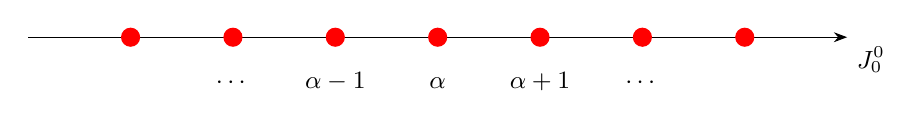
\begin{tikzpicture}[scale=0.65, font=\small]
            \draw[-{Stealth}] (-8, 0) -- (8, 0) node[anchor=north west] {$J_0^0$};

          \foreach \x / \labelText in {
              -6/{},
              -4/{\cdots}, 
              -2/{\alpha-1}, 
              0/{\alpha}, 
              2/{\alpha+1}, 
              4/{\cdots},
              6/{}
          } {
              \filldraw[red] (\x, 0) circle (5pt);
              
              \node[anchor=base] at (\x, -1) {$\labelText$};
          }

        \end{tikzpicture}
        \caption{$\mathcal{C}^{j}_{\alpha}$}
        \label{fig:nC}
    \end{subfigure}

    \vspace{1cm}
    \begin{subfigure}[b]{0.9\textwidth}
        \centering
        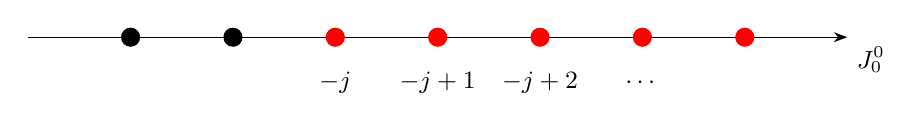
\begin{tikzpicture}[scale=0.65, font=\small]
            \draw[-{Stealth}] (-8, 0) -- (8, 0) node[anchor=north west] {$J_0^0$};

          \foreach \x / \labelText in {
              -2/{-j}, 
              0/{-j+1}, 
              2/{-j+2}, 
              4/{\cdots},
              6/{}
          } {
              \filldraw[red] (\x, 0) circle (5pt);
              
              \node[anchor=base] at (\x, -1) {$\labelText$};
          }

          \foreach \x / \labelText in {
              -6/{},
              -4/{}
          } {
              \filldraw[black] (\x, 0) circle (5pt);
              
              \node[anchor=base] at (\x, -1) {$\labelText$};
          }

        \end{tikzpicture}
        \caption{$\mathcal{D}^{j,+}$}
        \label{fig:nD+}
    \end{subfigure}

    \vspace{1cm}

    \begin{subfigure}[b]{0.9\textwidth}
        \centering
        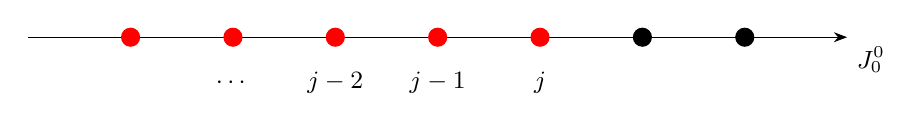
\begin{tikzpicture}[scale=0.65, font=\small]
            \draw[-{Stealth}] (-8, 0) -- (8, 0) node[anchor=north west] {$J_0^0$};

          \foreach \x / \labelText in {
              -6/{},
              -4/{\cdots}, 
              -2/{j-2}, 
              0/{j-1}, 
              2/{j}
          } {
              \filldraw[red] (\x, 0) circle (5pt);
              
              \node[anchor=base] at (\x, -1) {$\labelText$};
          }

          \foreach \x / \labelText in {
              4/{},
              6/{}
          } {
              \filldraw[black] (\x, 0) circle (5pt);
              
              \node[anchor=base] at (\x, -1) {$\labelText$};
          }

        \end{tikzpicture}
        \caption{$\mathcal{D}^{j,-}$}
        \label{fig:nD-}
    \end{subfigure}

    \vspace{1cm}

    \begin{subfigure}[b]{0.9\textwidth}
        \centering
        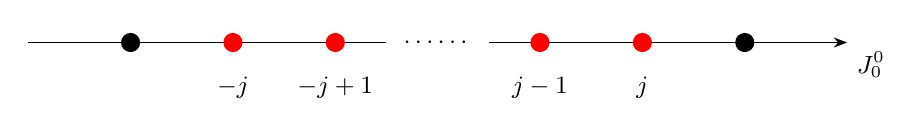
\begin{tikzpicture}[scale=0.65, font=\small]

          \draw (-8, 0) -- (-1, 0);

          \draw[-{Stealth}] (1, 0) -- (8, 0) node[anchor=north west] {$J^{0}_{0}$};

          \node at (0, 0) {$\cdots\cdots$};

          \foreach \x / \labelText in {
              -4/{-j},
              -2/{-j+1},
              2/{j-1},
              4/{j}
          } {
              \filldraw[red] (\x, 0) circle (5pt);
              
              \node[anchor=base] at (\x, -1) {$\labelText$};
          }

          \foreach \x / \labelText in {
              -6/{},
              6/{}
          } {
              \filldraw[black] (\x, 0) circle (5pt);
              
              \node[anchor=base] at (\x, -1) {$\labelText$};
          }
          
      \end{tikzpicture}
    \caption{$\mathcal{E}^{j}$}
    \label{fig:nE}
    \end{subfigure}

    \caption{The spectra of irreducible representations of $\mathfrak{sl}_{2}$}
    \label{fig:sl2}
\end{figure}

There is an outer automorphism in group $SL_{2}(\mathbb{R})$, namely the conjugation, which send the Lie algebra generators to 
\begin{equation}
    \left(J^{0}_{0}\right)^{*} = - J^{0}_{0} \quad \left(J^{\pm}_{0}\right)^{*} = - J^{\mp}_{0}.
\end{equation}
Composing a representation with the outer morphism, we obtain the so-called conjugate representation. The conjugation representation 
has the same spin and opposite $J^{0}_{0}$ eigenvalues:
\begin{equation}
    \left(\mathcal{C}^{j}_{\alpha}\right)^{*} = \mathcal{C}^{j}_{-\alpha} \quad \left(\mathcal{D}^{j,\pm}\right)^{*} = \mathcal{D}^{j,\mp}.
\end{equation}

\subsubsection*{Affine highest representations}
An affine highest-weight representation $\widehat{\mathcal{R}}$ of affine Lie algebra $\widehat{\mathfrak{g}}$ is defined by the action 
of $\widehat{\mathfrak{g}}$ on a affine highest-weight state $\ket{v}$. Hence if 
affine primary states $\ket{v^{\mathcal{R}}}$ transform in the representation $\mathcal{R}$ of the horizontal algebra $\mathfrak{g}$,
acting on the affine primary states with creation operators $J^{a}_{n<0}$ extends $\mathcal{R}$ to affine highest-weight representation 
$\widehat{\mathcal{R}}$. For an irreducible representation $\mathcal{R}$, the deduced affine 
highest-weight representation $\widehat{\mathcal{R}}$ is not necessarily irreducible.

From the above representations of $\mathfrak{sl}_{2}$, we can naturally induce the corresponding representations of $\widehat{\mathfrak{sl}_{2}}$. 
We plot the states by their eigenvalues of $L_{0}$ and $J^{0}_{0}$ in figure \ref{fig:irrep}.

\newpage

\begin{figure}[h]
    \centering 
    \begin{subfigure}[b]{0.48\textwidth}
        \centering
        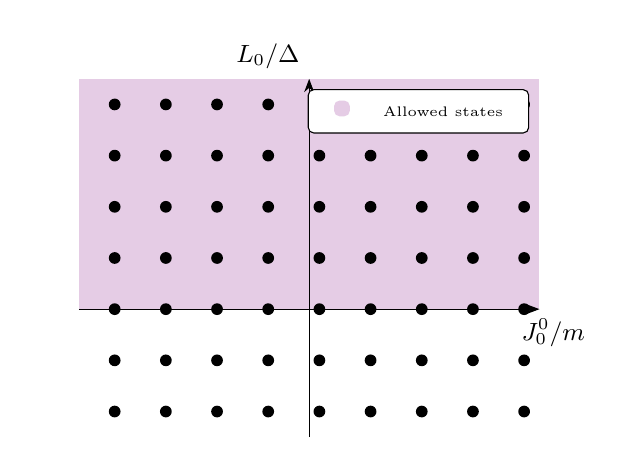
\begin{tikzpicture}[scale=0.65, font=\small]
            \def\xmin{-4.5} \def\xmax{4.5} \def\ymin{-2.5} \def\ymax{4.5}
            \clip (\xmin-1, \ymin) rectangle (\xmax+1, \ymax+1);
            
            \fill[violet!20] (\xmin, 0) rectangle (\xmax, \ymax);
            
            \draw[-{Stealth[]}] (\xmin, 0) -- (\xmax, 0) node[anchor=north west, xshift=-10pt] {$J_0^0/m$};
            \draw[-{Stealth[]}] (0, \ymin) -- (0, \ymax) node[anchor=south east] {$L_0/\Delta$};
            \foreach \x in {-4,...,4} {\foreach \y in {-2,...,4} {\node[dot] at (\x+0.2,\y) {};}}
                        
            \node[draw, fill=white, rounded corners=2pt, align=left, anchor=north east, font=\tiny] at (\xmax-0.2, \ymax-0.2) {
                \begin{tabular}{rl}\tikz\fill[violet!20](0,0)rectangle(0.2,0.2);&Allowed states\end{tabular}};
        \end{tikzpicture}
        \caption{$\widehat{\mathcal{C}}^{j}_{\alpha}$}
        \label{fig:C}
    \end{subfigure}
    \hfill 
    % (b) 右上角子图: V形边界
    \begin{subfigure}[b]{0.48\textwidth}
        \centering
        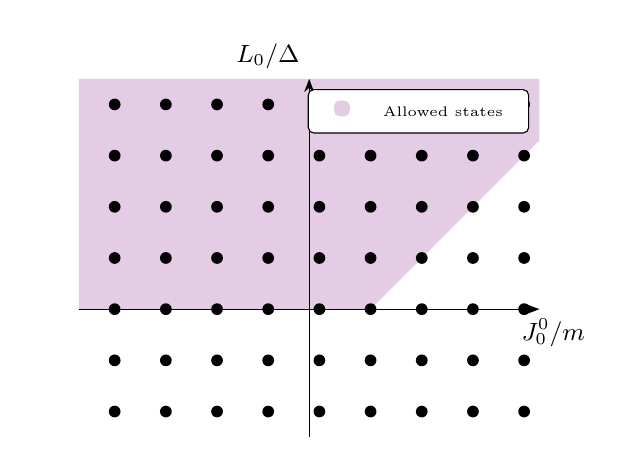
\begin{tikzpicture}[scale=0.65, font=\small]
            \def\xmin{-4.5} \def\xmax{4.5} \def\ymin{-2.5} \def\ymax{4.5}
            \clip (\xmin-1, \ymin) rectangle (\xmax+1, \ymax+1);

            \fill[violet!20] (\xmin, 0) -- (1.2, 0) -- (\xmax, \xmax-1.2) -- (\xmax, \ymax) -- (\xmin, \ymax) -- cycle;
            
            \draw[-{Stealth[]}] (\xmin, 0) -- (\xmax, 0) node[anchor=north west, xshift=-10pt] {$J_0^0/m$};
            \draw[-{Stealth[]}] (0, \ymin) -- (0, \ymax) node[anchor=south east] {$L_0/\Delta$};
            \foreach \x in {-4,...,4} {\foreach \y in {-2,...,4} {\node[dot] at (\x+0.2,\y) {};}}            
            
            \node[draw, fill=white, rounded corners=2pt, align=left, anchor=north east, font=\tiny] at (\xmax-0.2, \ymax-0.2) {
                \begin{tabular}{rl}\tikz\fill[violet!20](0,0)rectangle(0.2,0.2);&Allowed states\end{tabular}};
        \end{tikzpicture}
        \caption{$\widehat{\mathcal{D}}^{j,-}$}
        \label{fig:D-}
    \end{subfigure}

    \vspace{1cm}

    %=====================================================
    % --- 第二行 ---
    %=====================================================

    % (c) 左下角子图: 倒V形边界
    \begin{subfigure}[b]{0.48\textwidth}
        \centering
        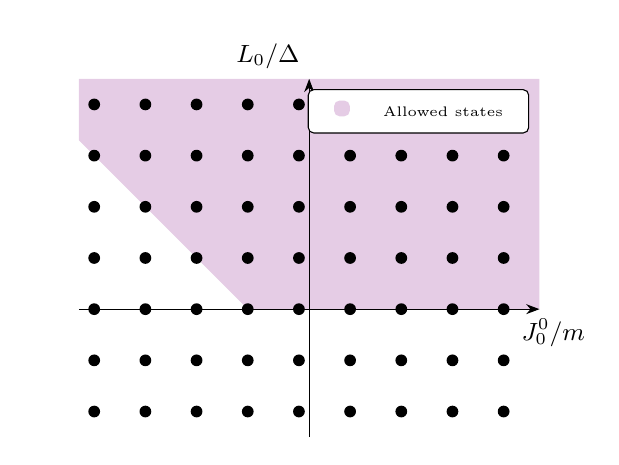
\begin{tikzpicture}[scale=0.65, font=\small]
            \def\xmin{-4.5} \def\xmax{4.5} \def\ymin{-2.5} \def\ymax{4.5}
            \clip (\xmin-1, \ymin) rectangle (\xmax+1, \ymax+1);

            \fill[violet!20] (\xmin, -\xmin-1.2) -- (-1.2, 0) -- (\xmax, 0) -- (\xmax, \ymax) -- (\xmin, \ymax) -- cycle;

            \draw[-{Stealth[]}] (\xmin, 0) -- (\xmax, 0) node[anchor=north west, xshift=-10pt] {$J_0^0/m$};
            \draw[-{Stealth[]}] (0, \ymin) -- (0, \ymax) node[anchor=south east] {$L_0/\Delta$};
            \foreach \x in {-4,...,4} {\foreach \y in {-2,...,4} {\node[dot] at (\x-0.2,\y) {};}}
                                    
            \node[draw, fill=white, rounded corners=2pt, align=left, anchor=north east, font=\tiny] at (\xmax-0.2, \ymax-0.2) {
                \begin{tabular}{rl}\tikz\fill[violet!20](0,0)rectangle(0.2,0.2);&Allowed states\end{tabular}};
        \end{tikzpicture}
        \caption{$\widehat{\mathcal{D}}^{j,+}$}
        \label{fig:D+}
    \end{subfigure}
    \hfill
    % (d) 右下角子图: 最终修正的复杂边界
    \begin{subfigure}[b]{0.48\textwidth}
        \centering
        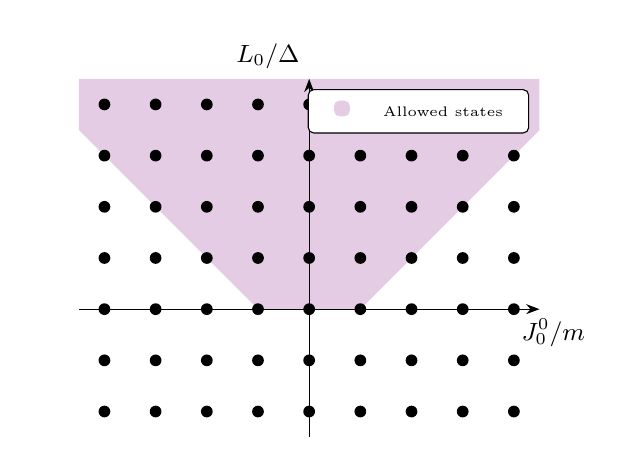
\begin{tikzpicture}[scale=0.65, font=\small]
            \def\xmin{-4.5} \def\xmax{4.5} \def\ymin{-2.5} \def\ymax{4.5}
            \clip (\xmin-1, \ymin) rectangle (\xmax+1, \ymax+1);

            \fill[violet!20] (\xmin, -\xmin-1) -- (-1, 0) -- (1, 0) -- (\xmax, \xmax-1) -- (\xmax, \ymax) -- (\xmin, \ymax) -- cycle;

            \draw[-{Stealth[]}] (\xmin, 0) -- (\xmax, 0) node[anchor=north west, xshift=-10pt] {$J_0^0/m$};
            \draw[-{Stealth[]}] (0, \ymin) -- (0, \ymax) node[anchor=south east] {$L_0/\Delta$};

            \foreach \x in {-4,...,4} {\foreach \y in {-2,...,4} {\node[dot] at (\x,\y) {};}}
            
            \node[draw, fill=white, rounded corners=2pt, align=left, anchor=north east, font=\tiny] at (\xmax-0.2, \ymax-0.2) {
                \begin{tabular}{rl}\tikz\fill[violet!20](0,0)rectangle(0.2,0.2);&Allowed states\end{tabular}};
        \end{tikzpicture}
    \caption{$\widehat{\mathcal{E}}^{j}$}
    \label{fig:E}
\end{subfigure}

    \caption{The spectra of irreducible representations of $\widehat{\mathfrak{sl}_{2}}$}
    \label{fig:irrep}
\end{figure}

\subsubsection*{Spectral flow}
The spectral flow is a family $(\rho_{\omega})_{\omega \in \mathbb{Z}}$ of automorphisms of $\widehat{\mathfrak{sl}_{2}}$
satisfying $\rho_{\omega_{1}} \circ \rho_{\omega_{2}}  = \rho_{\omega_{1} + \omega_{2}}$, which are defined by 
\begin{equation}
    \begin{aligned}
        \rho_{\omega}(J^{\pm}_{m}) & = J^{\pm}_{m \pm \omega},\\
        \rho_{\omega}(J^{0}_{m}) & = J^{0}_{m} + \frac{1}{2} k \omega \delta_{m,0}.
    \end{aligned}
\end{equation}
According to the Sugawara construction \eqref{DefLn}, the spectral flow of Virasoro generators is 
\begin{equation}
    \rho_{\omega}(L_{m}) = L_{m} + \omega J^{0}_{m} + \frac{1}{4} k n^{2} \delta_{m,0}.
\end{equation}
Hence the conformal dimension of a spectral flowed primary field $\phi^{j,\omega}_{m}(z)$ is 
\begin{equation}
    \Delta^{j,\omega}_{m} = \Delta_{j} - \omega m - \frac{1}{4} k m^{2}. \label{SpecFlowConDim}
\end{equation}

A representation $\widehat{\mathcal{R}} $ provides the action of generators $J^{a}_{n}$ on vector space $V$. Based on this representation, 
we define the spectral flowed representation $\rho_{\omega}\left(\widehat{\mathcal{R}}\right)$. The spectral flowed representation acts on the 
same vector space $V$, but the action of generators $J^{a}_{n}$ is defined to be $\rho_{-\omega}\left(J^{a}_{n}\right)$. 

For clarity in calculations, we label the states in $\rho_{\omega}\left(\widehat{\mathcal{R}}\right)$ by $\ket{j,m,\omega}$. The definition 
of the action of generators $J^{a}_{n}$ leads to
\begin{equation}
    J^{a}_{n} \ket{j,m,\omega} \equiv \rho^{-\omega} \left(J^{a}_{n}\right) \ket{j,m},
\end{equation}
where we omit the label $0$ in state $\ket{j,m,0}$ for simplicity. 
The conjugate representation of $\rho_{n} \left(\widehat{\mathcal{R}} \right)$ is 
\begin{equation}
    \rho_{\omega} \left( \widehat{\mathcal{R}} \right)^{*} = \rho_{-\omega} \left(\widehat{\mathcal{R}}^{*} \right).
\end{equation}

Let's consider the action of spectral flow on affine highest-weight representations. We introduce the following notation 
\begin{equation}
    \begin{aligned}
        \hat{\mathcal{C}}^{j,\omega} &= \rho_{\omega} \left( \hat{\mathcal{C}}^{j} \right),\\
        \hat{\mathcal{D}}^{j, \frac{1}{2} + \omega} &= \rho_{\omega} \left( \hat{\mathcal{D}}^{j, +} \right).
    \end{aligned} \label{SpecFlowNotation}
\end{equation}
From \eqref{SpecFlowConDim}, we find the conformal dimension of states in $\hat{\mathcal{C}}^{j,\omega}$ of non-zero $\omega$ are not bounded 
from below. Hence it cannot be an affine highest-weight representation.

On the other hand, the representations $\hat{\mathcal{D}}^{j,\pm}$ are characterized by the existence of state $\ket{j,\mp j}$, 
which satisfy the following conditions:
\begin{equation}
    J^{a}_{n>0} \ket{j,\pm j} = J^{\pm}_{0} \ket{j,\pm j} = (J^{0}_{0} \mp j) \ket{j,\pm j} =0.
\end{equation}
In particular, we notice that 
\begin{equation}
    \begin{aligned}
        J^{+}_{n \geq 0} \ket{j,-j,-1} &= J^{+}_{n+1} \ket{j,-j}  = 0, \\
        J^{0}_{n > 0} \ket{j,-j,-1} & =  J^{0}_{n}\ket{j,-j} = 0,\\
        \left(J^{0}_{0} - \frac{k}{2} +j \right) & = \left( J^{0}_{0} + j \right) \ket{j,-j} = 0,
        J^{-}_{n>0} \ket{j,-j,-1} &= J^{-}_{n-1} \ket{j,-j}   =  0.
    \end{aligned}
\end{equation}
Hence we find $\ket{j,-j,-1} = \ket{\frac{k}{2}-j, \frac{k}{2}-j}$, and 
\begin{equation}
    \hat{\mathcal{D}}^{j,-\frac{1}{2}} = \rho_{-1} \left( \hat{\mathcal{D}}^{j,+} \right) = \hat{\mathcal{D}}^{\frac{k}{2}-j,-}.
\end{equation}
Now we can use \eqref{SpecFlowNotation} to write the discrete series representations as 
\begin{equation}
    \widehat{\mathcal{D}}^{j,+} = \widehat{\mathcal{D}}^{j,\frac{1}{2}},\quad \widehat{\mathcal{D}}^{j,-} = \widehat{\mathcal{D}}^{\frac{k}{2}-j,-\frac{1}{2}}.
\end{equation}

Since the eigenvalue of $L_{0}$ are related to $m$, the spectrum of spectral flowed representations 
are twisted. We plot the spectrum of $\widehat{\mathcal{C}}^{j,1}_{\alpha}$ and $\widehat{\mathcal{D}}^{\frac{k}{2}-j, -\frac{1}{2}}$ 
in \ref{fig:irrepSF}.

\begin{figure}[htbp]
    \centering 
    \begin{subfigure}[b]{0.48\textwidth}
        \centering
        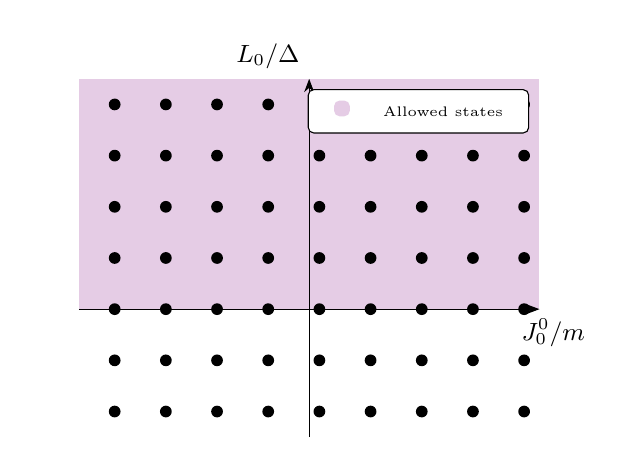
\begin{tikzpicture}[scale=0.65, font=\small]
            \def\xmin{-4.5} \def\xmax{4.5} \def\ymin{-2.5} \def\ymax{4.5}
            \clip (\xmin-1, \ymin) rectangle (\xmax+1, \ymax+1);
            
            \fill[violet!20] (\xmin, 0) rectangle (\xmax, \ymax);            

            \draw[-{Stealth[]}] (\xmin, 0) -- (\xmax, 0) node[anchor=north west, xshift=-10pt] {$J_0^0/m$};
            \draw[-{Stealth[]}] (0, \ymin) -- (0, \ymax) node[anchor=south east] {$L_0/\Delta$};
            \foreach \x in {-4,...,4} {\foreach \y in {-2,...,4} {\node[dot] at (\x+0.2,\y) {};}}
                        
            \node[draw, fill=white, rounded corners=2pt, align=left, anchor=north east, font=\tiny] at (\xmax-0.2, \ymax-0.2) {
                \begin{tabular}{rl}\tikz\fill[violet!20](0,0)rectangle(0.2,0.2);&Allowed states\end{tabular}};
        \end{tikzpicture}
        \caption{$\widehat{\mathcal{C}}^{j}_{\alpha}$}
        \label{fig:C0}
    \end{subfigure}
    \hfill 
%second picture at up-right corner
    \begin{subfigure}[b]{0.48\textwidth}
        \centering
        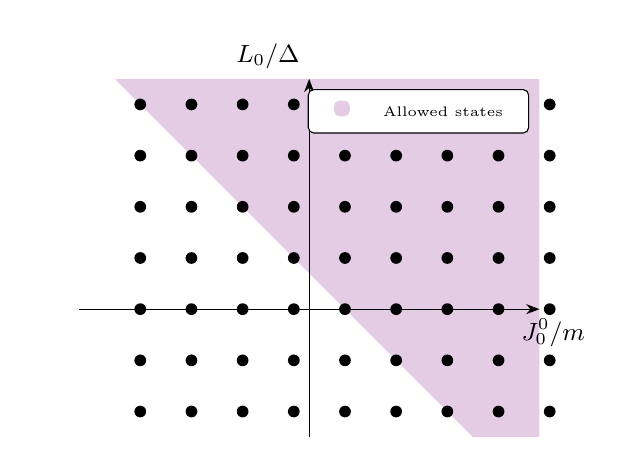
\begin{tikzpicture}[scale=0.65, font=\small]
            
            \def\xmin{-4.5} \def\xmax{4.5} \def\ymin{-2.5} \def\ymax{4.5}
            \clip (\xmin-1, \ymin) rectangle (\xmax+1, \ymax+1);

            \fill[violet!20] (-\ymax+0.7, \ymax) -- (-\ymin+0.7, \ymin) -- (\xmax, \ymin) -- (\xmax, \ymax) -- cycle;
            
            \draw[-{Stealth[]}] (\xmin, 0) -- (\xmax, 0) node[anchor=north west, xshift=-10pt] {$J_0^0/m$};
            \draw[-{Stealth[]}] (0, \ymin) -- (0, \ymax) node[anchor=south east] {$L_0/\Delta$};
            \foreach \x in {-4,...,4} {\foreach \y in {-2,...,4} {\node[dot] at (\x+0.2+0.5,\y) {};}}            
            
            \node[draw, fill=white, rounded corners=2pt, align=left, anchor=north east, font=\tiny] at (\xmax-0.2, \ymax-0.2) {
                \begin{tabular}{rl}\tikz\fill[violet!20](0,0)rectangle(0.2,0.2);&Allowed states\end{tabular}};
        \end{tikzpicture}
        \caption{$\widehat{\mathcal{C}}^{j,1}_{\alpha}$}
        \label{fig:C1}
    \end{subfigure}

    \vspace{1cm}

    %=====================================================
    % --- 第二行 ---
    %=====================================================

    \begin{subfigure}[b]{0.48\textwidth}
        \centering
        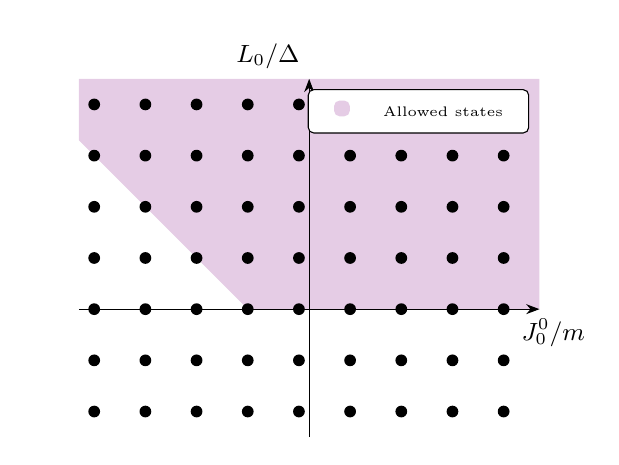
\begin{tikzpicture}[scale=0.65, font=\small]
            \def\xmin{-4.5} \def\xmax{4.5} \def\ymin{-2.5} \def\ymax{4.5}
            \clip (\xmin-1, \ymin) rectangle (\xmax+1, \ymax+1);

            \fill[violet!20] (\xmin, -\xmin-1.2) -- (-1.2, 0) -- (\xmax, 0) -- (\xmax, \ymax) -- (\xmin, \ymax) -- cycle;

            \draw[-{Stealth[]}] (\xmin, 0) -- (\xmax, 0) node[anchor=north west, xshift=-10pt] {$J_0^0/m$};
            \draw[-{Stealth[]}] (0, \ymin) -- (0, \ymax) node[anchor=south east] {$L_0/\Delta$};
            \foreach \x in {-4,...,4} {\foreach \y in {-2,...,4} {\node[dot] at (\x-0.2,\y) {};}}
                                    
            \node[draw, fill=white, rounded corners=2pt, align=left, anchor=north east, font=\tiny] at (\xmax-0.2, \ymax-0.2) {
                \begin{tabular}{rl}\tikz\fill[violet!20](0,0)rectangle(0.2,0.2);&Allowed states\end{tabular}};
        \end{tikzpicture}
        \caption{$\widehat{\mathcal{D}}^{j,\frac{1}{2}}$}
        \label{fig:D 1/2}
    \end{subfigure}
    \hfill
%fourth picture at down-right corner
    \begin{subfigure}[b]{0.48\textwidth}
        \centering
        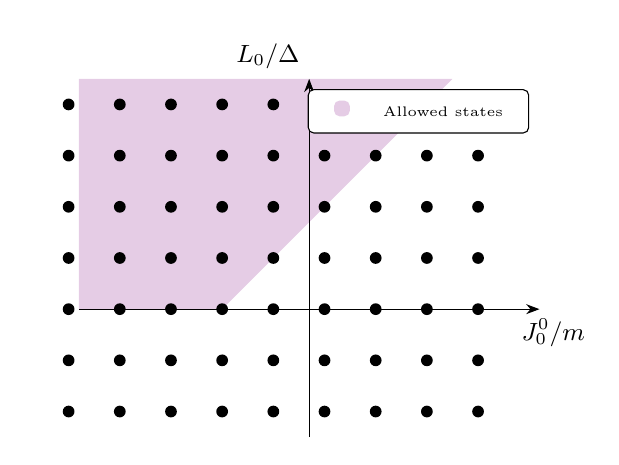
\begin{tikzpicture}[scale=0.65, font=\small]
            \def\xmin{-4.5} \def\xmax{4.5} \def\ymin{-2.5} \def\ymax{4.5}
            \clip (\xmin-1, \ymin) rectangle (\xmax+1, \ymax+1);

            \fill[violet!20] (\xmin, 0) -- (-1.7, 0) -- (\ymax-1.7, \ymax) -- (\xmin, \ymax) -- cycle;
            
            \draw[-{Stealth[]}] (\xmin, 0) -- (\xmax, 0) node[anchor=north west, xshift=-10pt] {$J_0^0/m$};
            \draw[-{Stealth[]}] (0, \ymin) -- (0, \ymax) node[anchor=south east] {$L_0/\Delta$};
            \foreach \x in {-4,...,4} {\foreach \y in {-2,...,4} {\node[dot] at (\x-0.7,\y) {};}}            
            
            \node[draw, fill=white, rounded corners=2pt, align=left, anchor=north east, font=\tiny] at (\xmax-0.2, \ymax-0.2) {
                \begin{tabular}{rl}\tikz\fill[violet!20](0,0)rectangle(0.2,0.2);&Allowed states\end{tabular}};
        \end{tikzpicture}
        \caption{$\widehat{\mathcal{D}}^{\frac{k}{2}-j, -\frac{1}{2}}$}
        \label{fig:D 1/2-1}
    \end{subfigure}

    \caption{Spectral flowed irreducible representations}
    \label{fig:irrepSF}
\end{figure}

\subsection{Correlation functions}

\subsubsection*{Ward identities}
The OPE \eqref{OPEJJ} implies the behaviour of $J^{a}(z)$ near $y = \infty$:
\begin{equation}
    \boxed{
        J^{a}(y) \underset{y \rightarrow \infty}{=} \mathcal{O}\left(\frac{1}{y^{2}}\right)
    }
\end{equation}
Consider a set of fields $\phi^{\sigma_{i}}(z_{i})$, and a meromorphic function $\epsilon(y)$ such that
$\epsilon(y) \underset{y \rightarrow \infty}{=} \mathcal{O}\left(1\right) $. Suppose $\epsilon(y)$
has no poles outside $\left\{z_{1},\cdots,z_{N} \right\}$, we have 
\begin{equation}
    \oint_{\infty} \mathrm{d} y \, \epsilon(y) \vev{J^{a}(y) \prod_{i} \phi^{\sigma}(z_{i})} = 0. \label{WardId}
\end{equation}
In case of $\epsilon(y) = 1$, we obtain the global Ward identities:
\begin{equation}
    \vev{\sum_{i} \left(J^{a}_{0}\right)^{(z_{i})} \prod_{i} \phi^{\sigma_{i}}(z_{i})} = 0,
\end{equation}
where $\left(J^{a}_{0}\right)^{(z_{i})}$ means the operator acts only on the $i$th field. Especially, if all the fields are affine primary 
fields, the global Ward identities reduce to 
\begin{equation}
    \sum_{i} D^{j_{i}}_{x}(t^{a}) \vev{\prod \phi^{j_{i}}_{x_{i}}(z_{i})} = 0. \label{GlobalWard}
\end{equation}
On the other hand, if we take $\epsilon(y) = \frac{1}{(y-z_{i})^{n}}$ and assume all fields but possibly the field at 
$z_{i}$ to be affine primary fields, we find the following local Ward identities:
\begin{equation}
    \vev{J^{a}_{-n} \phi^{\sigma_{i}}(z_{i}) \prod_{k \neq i} \phi^{j_{k}}_{x_{k}}(z_{k})} = \sum_{k\neq i} \frac{D^{j_{k}}_{x}(t^{a})}{(z_{k}-z_{i})^{n}} \vev{ \phi^{\sigma_{i}}(z_{i}) \prod_{k \neq i} \phi^{j_{k}}_{x_{k}}(z_{k})} \label{LocalWard}
\end{equation}

\subsubsection*{Three-point functions}
So far, we have only considered the chiral field $\phi^{j}(z)$ belongs to some representation $\widehat{\mathcal{R}^{j}}$ of 
$\widehat{\mathfrak{sl}_{2}}$. However, since the $\widetilde{SL}_{2}(\mathbb{R})$ WZW model is a CFT with $\widehat{\mathfrak{sl}_{2}}\times\widehat{\mathfrak{sl}_{2}}$ 
symmetry, the field $\phi^{j}(z,\bar{z})$ transforms under both $\widehat{\mathfrak{sl}_{2}}$ algebras. One may assume that 
the fields are a product $\phi^{j}(z,\bar{z}) \sim \phi^{j}(z)\phi^{j}(\bar{z})$ of chiral fields. However, this chiral 
factorization fails at the level of zero modes. Hence we need to construct the correlation functions with both holomorphic and anti-holomorphic 
parts.

When considreing both the left-moving and right-moving parts, the transformation between $x$-basis and $\mu$-basis is then given by 
\begin{equation}
    \phi^{j}_{x,\bar{x}}(z,\bar{z}) = \int_{\mathbb{C}} \mathrm{d}^{2} \mu \, |\mu|^{-2j-2} \mathrm{e}^{\mu x - \bar{\mu} \bar{x}} \phi^{j}_{\mu,\bar{\mu}}(z,\bar{z}).
\end{equation}
The fields in the $m$-basis are related to the $\mu$-basis fields by 
\begin{equation}
    \phi^{j}_{m,\bar{m}}(z,\bar{z}) = N^{j}_{m,\bar{m}} \int_{\mathbb{C}} \frac{\mathrm{d}^{2} \mu }{|\mu|^{2}} \, \mu^{-m} \bar{\mu}^{-\bar{m}} \phi^{j}_{\mu,\bar{\mu}} (z,\bar{z}).
\end{equation}
where the normalization factor is 
\begin{equation}
    N^{j}_{m,\bar{m}} = \frac{\Gamma(j+1-m)}{\Gamma(\bar{m} - j)}.
\end{equation} 
We use the following notation:
\begin{equation}
    \left| F(z,m) \right|^{2} = F(z,m) \times F(\bar{z},\bar{m}).
\end{equation}
Note that although $\bar{z}$ is the complex conjugate of $z$, $\bar{m}$ is not necessarily the complex conjugate of $m$. 

The 3-point functions with only affine primary fields can be determined from the global Ward identities \eqref{GlobalWard}. 
In the $x$-basis, we find the solution to be:
\begin{equation}
    \begin{aligned}
            \vev{\phi^{j_{1}}_{x_{1},\bar{x}_{1}}(z_{1},\bar{z}_{1}) \phi^{j_{2}}_{x_{2},\bar{x}_{2}}(z_{2},\bar{z}_{2}) \phi^{j_{3}}_{x_{3},\bar{x}_{3}}(z_{3},\bar{z}_{3})} = &
            |z_{12}|^{-2 \Delta_{12}^{3}} |z_{23}|^{-2 \Delta_{23}^{1}} |z_{31}|^{-2 \Delta_{31}^{2}} \\
            & \times D \left[\begin{array}{ccc}
    j_{1} & j_{2} & j_{3} \\
    x_{1} & x_{2} & x_{3}
    \end{array} \right] C(j_{1},j_{2},j_{3}),
    \end{aligned} \label{3pointfuncx}
\end{equation}
where $z_{ij} = z_{i} - z_{j}$ and $\Delta^{K}_{I} = \sum_{i \in I} \Delta_{j_{i}} - \sum_{k \in K} \Delta_{j_{k}}$. The structure constant 
$C(j_{1},j_{2},j_{3})$ is not fully determined yet. The x-dependence is included in the factor:
\begin{equation}
    D \left[\begin{array}{ccc}
    j_{1} & j_{2} & j_{3} \\
    x_{1} & x_{2} & x_{3}
    \end{array} \right] = |x_{12}|^{2 j_{12}^{3}} |x_{23}|^{2 j_{23}^{1}} |x_{31}|^{2 j_{31}^{2}}.
\end{equation}
In the $\mu$-basis, the corresponding factor is 
\begin{equation}
    \begin{aligned}
        D \left[\begin{array}{ccc}
        j_{1} & j_{2} & j_{3} \\
        \mu_{1} & \mu_{2} & \mu_{3}
        \end{array} \right] = & \pi |\mu_{2}|^{-2 j_{1} - 2 j_{3} - 2} |\mu_{1}|^{2j_{1} + 2} |\mu_{3}|^{2j_{3} + 2} \\
                            & \times \left[\frac{\gamma(j_{23}^{1} + 1) \gamma(j_{13}^{2} + 1)}{\gamma(-j_{123}-1) \gamma(2j_{3}+2)} {}_{2} \mathcal{F}_{1} (j_{123} +2, j_{13}^{2} +1, 2j_{3} + 2, -\frac{\mu_{3}}{\mu_{2}}) \right.\\
                            &\quad + \left. \left| \frac{-\mu_{3}}{\mu_{2}}\right|^{-2(2j_{3}+1)} \frac{\gamma(j_{12}^{3} + 1)}{\gamma(-2 j_{3})} {}_{2} \mathcal{F}_{1} (-j_{23}^{1}, j_{12}^{3} +1, -2j_{3}, -\frac{\mu_{3}}{\mu_{2}}) \right]
    \end{aligned}
\end{equation}
where ${}_{2} \mathcal{F}_{1}$ is the product of two hypergeometric functions, 
\begin{equation}
    {}_{2}\mathcal{F}_{1}(a,b,c,z) = F(a,b,c,z) \times F(a,b,c,\bar{z}).
\end{equation}
The factor $\gamma$ is defined by the gamma function 
\begin{equation}
    \gamma(x) = \frac{\Gamma(x)}{\Gamma(1-x)}.
\end{equation}

\subsubsection*{Three-point functions with spectral flow violation}
So far we have only discussed the 3-point function with affine primary fields. However, the spectral flow is not necessarily preserved 
under the fusion. In the OPE between two affine primary fields, the spectral flow can be violated by at most 1 unit: 
\begin{equation}
    \phi^{j_{1}}(z_{1}) \phi^{j_{2}}(z_{2}) \supset \sum_{j,\pm} \phi^{j,\pm 1}(z_{2}).
\end{equation}
In the $n$-point function, we can fuse the fields one by one and we find that the spectral flow can violate by at most $n-2$ units. 
To understand the full set of fusion rules, we must therefore consider these spectral flow violating correlation functions.

The simplest non-trivial case is a three-point function where the total spectral flows are $\sum_{i} \omega_{i} = \pm 1$. 
Let us consider the case where one field is flowed, e.g., $\vev{\phi^{j_{1}}(z_{1}) \phi^{j_{2}}(z_{2}) \phi^{j_{3},1}(z_{3})}$. 

The action of $J^{+}_{0}$ on spectral flowed field $\phi^{j,1}(z)$ is 
\begin{equation}
    J^{+}_{0}\phi^{j,1}(z) = \rho_{1} \left(J^{+}_{-1} \phi^{j}(z)\right),
\end{equation}
hence the $J^{+}_{0}$ global Ward identity will 
not give effective constraints on the 3-point function. On the other hand, since $J^{-}_{0} \phi^{j,1}(z) = 0$, 
the $J^{-}_{0}$ global Ward identity becomes: 
\begin{equation}
    \vev{J^{-}_{0} \phi^{j_{1}}(z_{1}) \phi^{j_{2}}(z_{2}) \phi^{j_{3},1}(z_{3})} + \vev{\phi^{j_{1}}(z_{1}) J^{-}_{0} \phi^{j_{2}}(z_{2}) \phi^{j_{3},1}(z_{3})}.
\end{equation}
In the $\mu$-basis, it means that 
\begin{equation}
    \mu_{1} + \mu_{2} = 0.
\end{equation}
In addition, the local Ward identity \eqref{LocalWard} for $J^{-}_{-1}$ now gives 
\begin{equation}
    \vev{ \phi^{j_{1}}_{\mu_{1}}(z_{1}) \phi^{j_{2}}_{\mu_{2}}(z_{2}) J^{-}_{-1} \phi^{j_{3},1}_{\mu_{3}}(z_{3})} 
    = \sum_{s=1,2} \frac{D^{j_{s}}_{\mu}(t^{-})}{z_{s}-z_{3}} \vev{ \phi^{j_{1}}_{\mu_{1}}(z_{1}) \phi^{j_{2}}_{\mu_{2}}(z_{2}) \phi^{j_{3},1}_{\mu_{3}}(z_{3})}.
\end{equation}
Hence we find 
\begin{equation}
    \frac{\mu_{1}}{z_{1}-z_{3}} + \frac{\mu_{2}}{z_{2}-z_{3}} + \mu_{3} = 0.
\end{equation}
Thus the 3-point function in the $\mu$-basis is proportional to 
$\delta(\mu_{1} + \mu_{2}) \delta\left(\frac{\mu_{1}}{z_{1}-z_{3}} + \frac{\mu_{2}}{z_{2}-z_{3}} + \mu_{3}\right)$.

The $z$-dependence of this 3-point function is given by \cite{Ribault:2005ms}, and the spectral flow violating 3-point function 
in the $\mu$-basis is 
\begin{equation}
    \begin{aligned}
        \vev{ \phi^{j_{1}}_{\mu_{1},\bar{\mu_{1}}}(z_{1},\bar{z_{1}}) \phi^{j_{2}}_{\mu_{2},\bar{\mu_{2}}}(z_{2},\bar{z_{2}}) \phi^{j_{3}}_{\mu_{3},\bar{\mu_{3}}}(z_{3},\bar{z_{3}})}
        = & |z_{12}|^{\frac{k}{2} -2-2\Delta^{3}_{12}} |z_{23}|^{\frac{k}{2} -2-2\Delta^{1}_{23}} |z_{31}|^{\frac{k}{2} -2-2\Delta^{2}_{31}}\\
        & \frac{1}{4 \pi^{2}} \delta^{2}(\mu_{1} + \mu_{2}) \delta^{2}\left(\frac{\mu_{1}}{z_{1}-z_{3}} + \frac{\mu_{2}}{z_{2}-z_{3}} + \mu_{3}\right)\\
        & \times \left| \frac{\mu_{1} z_{1}^{2}}{z_{1}-z_{3}} + \frac{\mu_{2} z_{2}^{2}}{z_{2}-z_{3}} + \mu_{3} z_{3}^{2} \right|^{4-k} C(j_{1},j_{2},j_{3}).
    \end{aligned}
\end{equation}
In the $m$-basis, the spectral flow violating 3-point function is 
\begin{equation}
    \begin{aligned}
        \vev{ \phi^{j_{1}}_{m_{1},\bar{m}_{1}}(z_{1},\bar{z_{1}}) \phi^{j_{2}}_{m_{2},\bar{m}_{2}}(z_{2},\bar{z_{2}}) 
        \phi^{j_{3},1}_{m_{3},\bar{m}_{3}}(z_{3},\bar{z_{3}}) } = \prod_{i} N^{j_{i}}_{m_{i},\bar{m}_{i}} \delta(\sum_{i} m_{i} - \frac{k}{2}) C(j_{1},j_{2},j_{3}) \\
        \times \left| z_{12}^{\Delta_{m_{3}}^{j_{3},\omega_{3}} -\Delta_{m_{1}}^{j_{1},\omega_{1}}-\Delta_{m_{2}}^{j_{2},\omega_{2}}} \, 
        z_{23}^{\Delta_{m_{1}}^{j_{1},\omega_{1}} -\Delta_{m_{2}}^{j_{2},\omega_{2}}-\Delta_{m_{3}}^{j_{3}} ,\omega_{3}} \, 
        z_{31}^{\Delta_{m_{2}}^{j_{2},\omega_{2}} -\Delta_{m_{3}}^{j_{3},\omega_{3}} -\Delta_{m_{1}}^{j_{1},\omega_{1}}}\right|^{2}
    \end{aligned} \label{3pointfunc_m-1}
\end{equation}
The 3-point function $\vev{ \phi^{j_{1}}_{m_{1},\bar{m}_{1}}(z_{1},\bar{z_{1}}) \phi^{j_{2}}_{m_{2},\bar{m}_{2}}(z_{2},\bar{z_{2}}) 
        \phi^{j_{3},-1}_{m_{3},\bar{m}_{3}}(z_{3},\bar{z_{3}}) } $ can be obtained similarly, and we find it is the same with \eqref{3pointfunc_m-1},
except that the selection rule is now $\delta(\sum_{i} m_{i} + \frac{k}{2})$. 

\section{Degenerate representations}
In addition to the irreducible representations, there exists a discrete set of representations known as the 
degenerate representations. Degenerate representations give constraints on the structure constant and hence play an essential role in 
making the model solvable. 

The defining feature of a degenerate representation is the vanishing of the null vectors (or null states) within its corresponding Verma module.
A descendant state $\ket{\chi} = \hat{N} \ket{j_{\hat{N}}} $ is called a null vector if it is also an affine primary state, which means 
that it is annihilated by all the positive mode currents:
\begin{equation}
    J^{a}_{n>0} \ket{\chi} = 0, \label{nullvectoreq}
\end{equation}
The existence of such a state implies that the representation $\widehat{\mathcal{V}}^{j}$ is reducible, 
as the null vector and its descendants form a non-trivial submodule $\widehat{\mathcal{V}}'$. 
The irreducible representation $\widehat{\mathcal{R}}^{j}$ is then obtained by taking the quotient of the Verma module by this submodule:
\begin{equation}
    \widehat{\mathcal{R}}^{j} = \frac{\widehat{\mathcal{V}}^{j}}{ \widehat{\mathcal{V}}'}
\end{equation}

At the level of fields, the field $\phi^{j_{\hat{N}}}$ corresponding to
$\ket{j_{\hat{N}}}$ is a degenerate field, which has a vanishing descendant 
\begin{equation}
    \hat{N} \phi^{j_{\hat{N}}} = 0.
\end{equation}
This null vector equation leads to differential equations for the correlation functions involving the corresponding degenerate field, then 
giving constraints on the correlation functions and the structure constants. 

The degenerate representations $\widehat{\mathcal{R}}^{\vev{r,s}}$ are labeled by two integers $r$ and $s$. The spin $j_{r,s}$ of 
degenerate representation $\widehat{\mathcal{R}}^{\vev{r,s}}$ is given by the following formula: 
\begin{equation}
    j_{\vev{r,s}} = \frac{s-1}{2} - \frac{k+2}{2} r \quad \mathrm{for} \quad s\geq 1, r \geq 0.
\end{equation}
The corresponding null vector is at level $N=rs$.

\subsection{Level 0 null vector}
The degenerate representation with a null vector at level 0 is of spin $j_{s} \equiv j_{\vev{0,s}}  = \frac{s-1}{2}$, which is nothing but the affine 
highest-weight extension of the finite dimensional representations. The $\widehat{\mathcal{R}}^{\vev{0,s}}$ contains a trivial null 
vector 
\begin{equation}
    J^{-}_{0} \ket{j_{s},-j_{s}} = 0.
\end{equation}

\subsection{Level 1 null vector}
The only possibility to have a level 1 null vector is $r = s = 1$, with $j_{\vev{1,1}} = -\frac{k+2}{2}$. 
The corresponding null vector is given in \cite{Stocco:2022gah}:
\begin{equation}
    \hat{N}^{c}_{1,1} = K_{ab} J^{a}_{-1} J^{b}_{0} J^{c}_{0} + j_{\vev{1,1}} f^{c}_{ab} J^{a}_{-1} J^{b}_{0} - 2 j^{2}_{\vev{1,1}} J^{c}_{-1}. \label{nullvector}
\end{equation}
We have no constraint on the $m$ of the null vector, hence the level 1 degenerate representation could belong to either 
principal continuous series or discrete series. This null vector satisfies the null vector equation \eqref{nullvectoreq}:
\begin{equation}
    \begin{aligned}
        J^{d}_{1} \hat{N}^{c}_{1,1} \ket{j_{\vev{1,1}},m}
        &= \left( K_{ab} \left[J^{d}_{1},J^{a}_{-1}\right] J^{b}_{0} J^{c}_{0} + j_{\vev{1,1}} f^{c}_{ab} \left[J^{d}_{1},J^{a}_{-1}\right] J^{b}_{0} - 2 j^{2}_{1,1} \left[J^{d}_{1},J^{c}_{-1}\right] \right)\ket{j_{\vev{1,1}},m} \\
        &= (2+k+2j_{\vev{1,1}})J^{d}_{0} J^{c}_{0} + (2j_{\vev{1,1}} + kj_{\vev{1,1}}+2j^{2}_{1,1})f^{ca}_{e} - K^{ac}j_{\vev{1,1}}(K_{eb}J^{e}_{0}J^{b}_{0}-2k j_{\vev{1,1}})\\
        &= 0,
    \end{aligned}
\end{equation}
where we use an identity $f^{ab}_{e} f^{ec}_{d} = 2(K^{a}_{d}K^{bc}- K^{ac}K^{b}_{d})$ that holds for $\mathfrak{sl}_{2}$, and 
the definition of Casimir operator $C = K_{ab} J^{a}_{0} J^{b}_{0} = 2j_{\vev{1,1}}(j_{\vev{1,1}}+1)$. On the other hand, the commutation relation 
between $J^{a}_{0}$ and $\hat{N}^{b}_{1,1}$ is 
\begin{equation}
    \left[ J^{a}_{0},\hat{N}^{b}_{1,1} \right] = f^{ab}_{c} \hat{N}^{c}_{1,1}. \label{CRJN}
\end{equation}
It implies the null vector $\hat{N}^{c}_{1,1} \ket{j_{\vev{1,1}}}$ generates a subrepresentation of $\widehat{\mathfrak{sl}_{2}}$.

\subsubsection*{Subrepresentations}

The states $\hat{N}^{+}_{1,1}\ket{j,m-1}$, $\hat{N}^{0}_{1,1}\ket{j,m}$, and $\hat{N}^{-}_{1,1} \ket{j,m+1}$ 
all have the same $J^{0}_{0}$ eigenvalue, namely $m$. We are interested in whether these three states are independent. 
These states can be expanded in the basis of $J^{a}_{-1}\ket{j_{\vev{1,1}},m}$. 
\begin{equation}
    \begin{aligned}
        \hat{N}^{+}_{1,1} \ket{j_{\vev{1,1}},m-1} = & ((j_{\vev{1,1}}-m+1)(j_{\vev{1,1}}+m) +2 j_{\vev{1,1}}(m-1) -2 j_{\vev{1,1}}^2) \, J^{+}_{-1}  \ket{j_{\vev{1,1}},m-1} \\
        & + (2(j_{\vev{1,1}}-m+1)m-2j_{\vev{1,1}}(j_{\vev{1,1}}-m+1)) \, J^{0}_{-1}  \ket{j_{\vev{1,1}},m} \\
        & + (j_{\vev{1,1}}-m+1)(j_{\vev{1,1}}-m) \, J^{-}_{-1} \ket{j_{\vev{1,1}},m+1}\\
        = & (j_{\vev{1,1}}+1+m)(-j_{\vev{1,1}}-m)\Big( J^{+}_{-1} \ket{j_{\vev{1,1}},m-1} + 2 J^{0}_{-1} \ket{j_{\vev{1,1}},m} - J^{-1}_{-1} \ket{j_{\vev{1,1}},m+1} \Big)\\
    \end{aligned} \label{nullvectorm}
\end{equation}
We define 
\begin{equation}
    \ket{N_{j}} \equiv J^{+}_{-1} \ket{j,m-1} + 2 J^{0}_{-1} \ket{j,m} - J^{-1}_{-1} \ket{j,m+1}.
\end{equation}
We find the other two states to be
\begin{equation}
    \hat{N}^{0}_{1,1} \ket{j_{\vev{1,1}},m} = -(j_{\vev{1,1}}-m)(m+j_{\vev{1,1}}) \ket{N_{j_{\vev{1,1}}}},
\end{equation}
\begin{equation}
    \hat{N}^{-}_{1,1} \ket{j_{\vev{1,1}},m+1} =  (j_{\vev{1,1}}+m)(j_{\vev{1,1}}+m+1) \ket{N_{j_{\vev{1,1}}}}.
\end{equation}
Hence all these three states are linearly dependent. 

To find the spin of the subrepresentation, we first calculate the eigenstates of the Casimir operator.
The commutation relation of Casimir operator with $J^{c}_{-1}$ is 
\begin{equation}
        \left[C,J^{c}_{-1}\right] = K_{ab}\left[J^{a}_{0}J^{b}_{0},J^{c}_{-1}\right]
        = -f^{c}_{bd} J^{d}_{-1}J^{b}_{0} - f^{c}_{bd}J^{b}_{0}J^{d}_{-1}
\end{equation}
The action of $C$ on basis $J^{a}_{-1} \ket{j,m}$ can be writen as the following matrix:
\begin{eqnarray}
    \begin{aligned}
        C 
    \begin{pmatrix}
    J^{+}_{-1} \ket{j,m-1}\\
    J^{0}_{-1} \ket{j,m}\\
    J^{-}_{-1} \ket{j,m+1}
    \end{pmatrix}
    = \begin{pmatrix}
        4m+2j(j+1) & -2 (-j-1+m) & 0\\
        -4 (-j-m) & 4 + 2j(j+1) & 4(-j+m)\\
        0 & 2 (-j-1-m)& -4m + 2j(j+1)
    \end{pmatrix}
    \begin{pmatrix}
        J^{+}_{-1} \ket{j,m-1}\\
        J^{0}_{-1} \ket{j,m}\\
        J^{-}_{-1} \ket{j,m+1}
    \end{pmatrix}
    \end{aligned}
\end{eqnarray}
After diagonalization, we find the eigenvectors and the corresponding eigenvalues are 
\begin{equation}
    \left\{
        \begin{aligned}
            j+1 &: -\frac{j+1-m}{j+m} J^{+}_{-1} \ket{j,m-1} + 2 J^{0}_{-1} \ket{j,m} + \frac{j+1+m}{j-m} J^{-}_{-1} \ket{j,m+1}\\
            j &: \frac{-j-1+m}{m} J^{+}_{-1} \ket{j,m-1} + 2 J^{0}_{-1} \ket{j,m} + \frac{-j-1-m}{m} J^{-}_{-1} \ket{j,m+1}\\
            j-1 &: J^{+}_{-1} \ket{j,m-1} + 2 J^{0}_{-1} \ket{j,m} - J^{-}_{-1} \ket{j,m+1} = \ket{N_{j}}.
        \end{aligned}
    \right.
\end{equation}
We find that $N_{1,1}\ket{j,m}$ is exactly the eigenvector corresponding to $j-1$. Hence the subrepresentation has spin $j_{\vev{1,1}}-1 = j_{1,-1}$.

\subsection{Spectral flowed degenerate representations}

For a given null vector $\ket{\chi}$, we could naturally define the spectral flowed null vector $\ket{\chi,\omega}$. 
It satisfies the flowed null vector equation automatically:
\begin{equation}
    \rho_{\omega} \left(J^{a}_{n>0}\right) \ket{\chi,\omega} = 0.
\end{equation}
We define a representation to be a spectral flowed degenerate representation if it contains a spectral flowed null vector, which can 
be obtained by applying spectral flow to the degenerate representations.

Since 
\begin{equation}
    \rho_{-1} \left( \widehat{\mathcal{D}}^{j,+} \right) = \widehat{\mathcal{D}}^{\frac{k}{2}-j,-},
\end{equation}
the spectral flowed degenerate representation $\rho_{-1} \left( \widehat{\mathcal{D}}^{\vev{r,s},+} \right)$ is also a affine highest-weight 
representation. On the other hand, we have 
\begin{equation}
    \frac{k}{2} - j_{\vev{r,s}} = \frac{k}{2} - \frac{s-1}{2} + \frac{k+2}{2} r = \frac{-s-1}{2} + \frac{k+2}{2}(r+1) = -j_{\vev{r+1,s}}-1.
\end{equation}
Hence we find
\begin{equation}
    \rho_{-1} \left( \widehat{\mathcal{D}}^{\vev{r,s},+} \right) = \widehat{\mathcal{D}}^{\vev{r+1,s},-},
\end{equation}
which means that the affine highest-weight degenerate representation $\widehat{\mathcal{D}}^{\vev{r,s},+}$ is itself a spectral flowed 
degenerate representation. A proof for $\vev{r,s} = \vev{1,1}$ will be given in the next section.

\subsubsection*{spectral flowed vacuum representation} 
Now we consider the spectral flow of the vacuum representation, i.e. of the degenerate representation $\widehat{\mathcal{E}}^{0}$. 
One could view $\widehat{\mathcal{E}}^{0}$ as
\begin{equation}
    \widehat{\mathcal{E}}^{0} = \hat{\mathcal{D}}^{\vev{0,1},+} = \hat{\mathcal{D}}^{\vev{0,1},-}
\end{equation}
which implies the following relation: 
\begin{equation}
    \begin{aligned}
        \rho_{1} \left(\widehat{\mathcal{E}}^{0}\right) &= \hat{\mathcal{D}}^{\vev{1,1},+}\\
        \rho_{-1} \left(\widehat{\mathcal{E}}^{0}\right) &= \hat{\mathcal{D}}^{\vev{1,1},-}.
    \end{aligned}
\end{equation}
We can verify that $\ket{0,0,-1}$ is indeed an affine highest-weight state:
\begin{equation}
    \begin{aligned}
        J^{+}_{1} \ket{0,0,-1} &= J^{+}_{2} \ket{0,0} = 0, \\
        J^{0}_{1} \ket{0,0,-1} &= J^{0}_{1} \ket{0,0} = 0, \\
        J^{-}_{1} \ket{0,0,-1} &= J^{-}_{0} \ket{0,0} = 0, 
    \end{aligned}
\end{equation}
In addition, we have 
\begin{equation}
    \begin{aligned}
        J^{+}_{0} \ket{0,0,-1} &= J^{+}_{1} \ket{0,0} = 0,\\
        J^{0}_{0} \ket{0,0,-1} &= \left(J^{0}_{0} + \frac{k}{2} \right) \ket{0,0} = \frac{k}{2} \ket{0,0}.
    \end{aligned}
\end{equation}
Hence we find 
\begin{equation}
    \ket{0,0,-1} = \ket{\frac{k}{2}, \frac{k}{2}}.
\end{equation}

\subsection{Spectra of degenerate representations}
We plot the spectra of degenerate representations as figure \ref{fig:degrep}. In these plots, each dot corresponds to eigenvalues of $J^{0}_{0}$ and 
$L_{0}$. The states appears in a representation are denoted by the shadowed area. The null vectors are labeled by the blue dashed line. 

\subsubsection*{Continuous series \texorpdfstring{$\widehat{\mathcal{C}}^{j}_{\alpha}$}{Lg}}
The spectrum of $\mathcal{C}^{j}_{\alpha}$ is unbounded, with eigenvalues of $m\in \alpha + \mathbb{Z}$. For each affine primary state 
$\ket{j,\alpha+m}$ at level 0, there is a corresponding null vector $\hat{N}^{0}_{1,1}$ live at level 1. 
Hence there is a straight line in the \ref{fig:C11_0}. 

After spectral flow, the eigenvalue of $L_{0}$ on $\ket{j,\alpha+m,1}$ is 
\begin{equation}
    L_{0} \ket{j,\alpha + m, 1} = \rho_{-1} \left(L_{0} \right) \ket{j,\alpha + m} = \left(\Delta_{j} - k + \frac{k^{2}}{4} \right) \ket{j,\alpha+m}.
\end{equation}
Hence the lower bound the spectrum is rotated, as well as the null states. The spectral flowed spectrum is plotted in 
figure \ref{fig:C11_1}.

\subsubsection*{Descrete series \texorpdfstring{$\widehat{\mathcal{D}}^{\vev{1,1},\frac{1}{2}}$}{D11}}
The spectrum of $\mathcal{D}^{\vev{1,1},\frac{1}{2}}$ is bounded from below, where there is a lowest weight state $\ket{j_{\vev{1,1}},-j_{\vev{1,1}}}$ in the spectrum of 
The subrepresentation at level 1 also has a lowest weight state. Since the spin of this subrepresentation is $j_{\vev{1,1}}-1$, the $J^{0}_{0}$ 
eigenvalue of this lowest weight state should be $1-j_{\vev{1,1}}$. hence the lowest weight state in the subrepresentation is 
$\hat{N}^{+}_{1,1} \ket{j_{\vev{1,1}},-j_{\vev{1,1}}}$, with the other two null vector $\hat{N}^{0}_{1,1} \ket{j_{\vev{1,1}},-j_{\vev{1,1}}}$ and 
$\hat{N}^{0}_{1,1} \ket{j_{\vev{1,1}},-j_{\vev{1,1}}}$ vanish, which implies 
\begin{equation}
    J^{-}_{0} \hat{N}^{+}_{1,1} \ket{j_{\vev{1,1}},-j_{\vev{1,1}}} = 0.
\end{equation}

On the other hand, the null state $\hat{N}^{+}_{1,1} \ket{j_{\vev{1,1}},-j_{\vev{1,1}}}$ is also an 
spectral flowed null state:
\begin{equation}
    \begin{aligned}
        \rho_{1} \left(J^{+}_{1} \right) \hat{N}^{+}_{1,1} \ket{j_{\vev{1,1}},-j_{\vev{1,1}}} &= 
        J^{+}_{2} \hat{N}^{+}_{1,1} \ket{j_{\vev{1,1}},-j_{\vev{1,1}}} = 0, \\
        \rho_{1} \left(J^{0}_{1} \right) \hat{N}^{+}_{1,1} \ket{j_{\vev{1,1}},-j_{\vev{1,1}}} &= 
        J^{0}_{1}  \hat{N}^{+}_{1,1} \ket{j_{\vev{1,1}},-j_{\vev{1,1}}} = 0, \\
        \rho_{1} \left(J^{-}_{1} \right) \hat{N}^{+}_{1,1} \ket{j_{\vev{1,1}},-j_{\vev{1,1}}} &= 
        J^{-}_{0}  \hat{N}^{+}_{1,1} \ket{j_{\vev{1,1}},-j_{\vev{1,1}}} = 0.
    \end{aligned}
\end{equation}
In addition, all states on the line $ \left(J^{-}_{-1}\right)^{n} \hat{N}^{+}_{1,1} \ket{j_{\vev{1,1}},-j_{\vev{1,1}}}, n\in \mathbb{N} $
are also spectral flowed null states, which can be proved by induction. Suppose 
$ \left(J^{-}_{-1}\right)^{n} \hat{N}^{+}_{1,1} \ket{j_{\vev{1,1}},-j_{\vev{1,1}}} $ 
is a spectral flowed null state, then we have
\begin{equation}
    \begin{aligned}
        \rho_{1} \left(J^{-}_{1} \right)  \left(J^{-}_{-1}\right)^{n+1} \hat{N}^{+}_{1,1} \ket{j_{\vev{1,1}},-j_{\vev{1,1}}}
        &= J^{-}_{0} \left(J^{-}_{-1}\right)^{n+1} \hat{N}^{+}_{1,1} \ket{j_{\vev{1,1}},-j_{\vev{1,1}}} \\
        &= \left(J^{-}_{-1}\right)^{n+1} J^{-}_{0} \hat{N}^{+}_{1,1} \ket{j_{\vev{1,1}},-j_{\vev{1,1}}} \\
        &=0.
    \end{aligned}
\end{equation}
For $J^{0}_{1}$, we have
\begin{equation}
    \begin{aligned}
        \rho_{1} \left(J^{0}_{1}\right) \left(J^{-}_{-1}\right)^{n+1} \hat{N}^{+}_{1,1} \ket{j_{\vev{1,1}},-j_{\vev{1,1}}}
        &= J^{0}_{1} \left(J^{-}_{-1}\right)^{n+1} \hat{N}^{+}_{1,1} \ket{j_{\vev{1,1}},-j_{\vev{1,1}}} \\
        &= J^{-}_{-1} J^{-}_{0} \left(J^{-}_{-1}\right)^{n} \hat{N}^{+}_{1,1} \ket{j_{\vev{1,1}},-j_{\vev{1,1}}} - J^{-}_{0} \left(J^{-}_{-1}\right)^{n} \hat{N}^{+}_{1,1} \ket{j_{\vev{1,1}},-j_{\vev{1,1}}} \\
        & = 0.
    \end{aligned}
\end{equation}
For $J^{+}_{1}$, we have
\begin{equation}
    \begin{aligned}
        \rho_{1} \left(J^{+}_{1}\right) \left(J^{-}_{-1}\right)^{n+1} \hat{N}^{+}_{1,1} \ket{j_{\vev{1,1}},-j_{\vev{1,1}}}
        &= J^{+}_{2} \left(J^{-}_{-1}\right)^{n+1} \hat{N}^{+}_{1,1} \ket{j_{\vev{1,1}},-j_{\vev{1,1}}} \\
        &= J^{-}_{-1} J^{+}_{2} \left(J^{-}_{-1}\right)^{n} \hat{N}^{+}_{1,1} \ket{j_{\vev{1,1}},-j_{\vev{1,1}}} + 2 J^{0}_{1} \left(J^{-}_{-1}\right)^{n} \hat{N}^{+}_{1,1} \ket{j_{\vev{1,1}},-j_{\vev{1,1}}} \\
        & = 0.
    \end{aligned}
\end{equation}
Hence we have another dashed line in figure \ref{fig:D 11_1}, which indicates that 
$\widehat{\mathcal{D}}^{\vev{1,1},+}$ is itself a spectral flowed degenerate representation: 
\begin{equation}
    \rho_{-1} \left( \widehat{\mathcal{D}}^{\vev{1,1},+} \right) = \widehat{\mathcal{D}}^{\vev{2,1},-}.
\end{equation}

After spectral flow, there are also a set of null states and another set of spectral flowed null states in the spectrum of 
$\widehat{\mathcal{D}}^{\vev{2,1},-}$. Hence we have two dashed lines in the figure \ref{fig:D 21_-1}.
Diagrammatically, the sets of null states are 'rotated' simultaneously.

\subsubsection*{Vacuum representation \texorpdfstring{$\widehat{\mathcal{E}}^{0}$}{Lg}}

Since the null vectors of the vacuum representation appears at level 0, the dashed line coincide with the axis $L_{0} = 0$, as shown in 
figure \ref{fig:E 1_0}. 

After the spectral flow, the null vector at level one is $J^{+}_{-1} \ket{\frac{k}{2}, \frac{k}{2}}$. There are two sets of the null vectors, 
namely $\left(J^{+}_{-1}\right)^{n} \ket{\frac{k}{2}, \frac{k}{2}}$ and $\left(J^{-}_{1}\right)^{n} \ket{\frac{k}{2}, \frac{k}{2}}$. However, 
since $\left(J^{-}_{1}\right)^{n} \ket{\frac{k}{2}, \frac{k}{2}}$ is outside of the spectrum, they are not plotted in figure \ref{fig:E 1_-1}.

\begin{figure}[htbp]
    \centering 
    \begin{subfigure}[b]{0.48\textwidth}
        \centering
        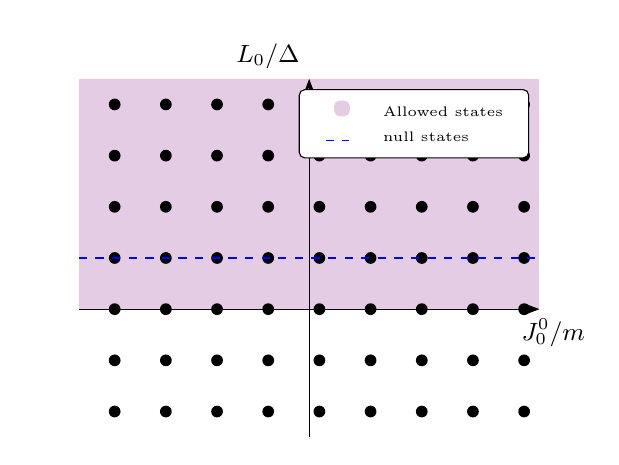
\begin{tikzpicture}[scale=0.65, font=\small]
            \def\xmin{-4.5} \def\xmax{4.5} \def\ymin{-2.5} \def\ymax{4.5}
            \clip (\xmin-1, \ymin) rectangle (\xmax+1, \ymax+1);
            
            \fill[violet!20] (\xmin, 0) rectangle (\xmax, \ymax);
            
            \draw[-{Stealth[]}] (\xmin, 0) -- (\xmax, 0) node[anchor=north west, xshift=-10pt] {$J_0^0/m$};
            \draw[-{Stealth[]}] (0, \ymin) -- (0, \ymax) node[anchor=south east] {$L_0/\Delta$};
            \foreach \x in {-4,...,4} {\foreach \y in {-2,...,4} {\node[dot] at (\x+0.2,\y) {};}}
            
            \draw[blue, dashed, thick] (\xmin, 1) -- (\xmax, 1);
    
            \node[draw, fill=white, rounded corners=2pt, align=left, anchor=north east, font=\tiny] at (\xmax-0.2, \ymax-0.2) {
                \begin{tabular}{rl}\tikz\fill[violet!20](0,0)rectangle(0.2,0.2);&Allowed states\\\tikz\draw[blue,dashed](0,0.1)--(0.3,0.1);&null states\\\end{tabular}};
        \end{tikzpicture}
        \caption{$\widehat{\mathcal{C}}^{\vev{1,1}}_{\alpha}$}
        \label{fig:C11_0}
    \end{subfigure}
    \hfill 
%second picture at up-right corner
    \begin{subfigure}[b]{0.48\textwidth}
        \centering
        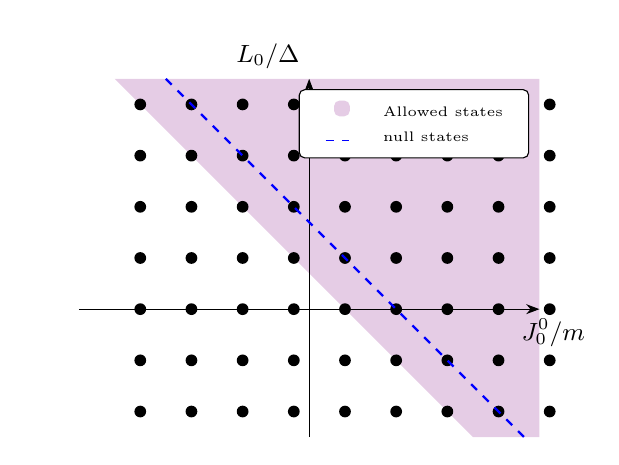
\begin{tikzpicture}[scale=0.65, font=\small]
            \def\xmin{-4.5} \def\xmax{4.5} \def\ymin{-2.5} \def\ymax{4.5}
            \clip (\xmin-1, \ymin) rectangle (\xmax+1, \ymax+1);

            \fill[violet!20] (-\ymax+0.7, \ymax) -- (-\ymin+0.7, \ymin) -- (\xmax, \ymin) -- (\xmax, \ymax) -- cycle;
            
            \draw[-{Stealth[]}] (\xmin, 0) -- (\xmax, 0) node[anchor=north west, xshift=-10pt] {$J_0^0/m$};
            \draw[-{Stealth[]}] (0, \ymin) -- (0, \ymax) node[anchor=south east] {$L_0/\Delta$};
            \foreach \x in {-4,...,4} {\foreach \y in {-2,...,4} {\node[dot] at (\x+0.2+0.5,\y) {};}}    
            
            \draw[blue, dashed, thick] (-\ymax+1.7, \ymax) -- (-\ymin+1.7, \ymin);
            
            \node[draw, fill=white, rounded corners=2pt, align=left, anchor=north east, font=\tiny] at (\xmax-0.2, \ymax-0.2) {
                \begin{tabular}{rl}\tikz\fill[violet!20](0,0)rectangle(0.2,0.2);&Allowed states\\\tikz\draw[blue,dashed](0,0.1)--(0.3,0.1);&null states\\\end{tabular}};
        \end{tikzpicture}
        \caption{$\widehat{\mathcal{C}}^{\vev{1,1},1}_{\alpha}$}
        \label{fig:C11_1}
    \end{subfigure}

    \vspace{1cm}

    %=====================================================
    % --- 第二行 ---
    %=====================================================

    \begin{subfigure}[b]{0.48\textwidth}
        \centering
        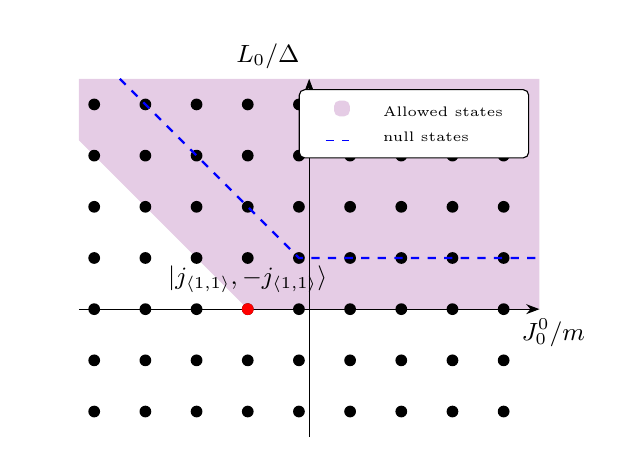
\begin{tikzpicture}[scale=0.65, font=\small]
            \def\xmin{-4.5} \def\xmax{4.5} \def\ymin{-2.5} \def\ymax{4.5}
            \clip (\xmin-1, \ymin) rectangle (\xmax+1, \ymax+1);

            \fill[violet!20] (\xmin, -\xmin-1.2) -- (-1.2, 0) -- (\xmax, 0) -- (\xmax, \ymax) -- (\xmin, \ymax) -- cycle;

            \draw[-{Stealth[]}] (\xmin, 0) -- (\xmax, 0) node[anchor=north west, xshift=-10pt] {$J_0^0/m$};
            \draw[-{Stealth[]}] (0, \ymin) -- (0, \ymax) node[anchor=south east] {$L_0/\Delta$};
            \foreach \x in {-4,...,4} {\foreach \y in {-2,...,4} {\node[dot] at (\x-0.2,\y) {};}}

            \draw[blue, dashed, thick] (-\ymax+0.8, \ymax) -- (-0.2, 1) -- (\xmax, 1) ;

            \node[dot, red, label=above:{$|j_{\vev{1,1}}, -j_{\vev{1,1}}\rangle$}] at (-1.2, 0) {};
    
            \node[draw, fill=white, rounded corners=2pt, align=left, anchor=north east, font=\tiny] at (\xmax-0.2, \ymax-0.2) {
                \begin{tabular}{rl}\tikz\fill[violet!20](0,0)rectangle(0.2,0.2);&Allowed states\\\tikz\draw[blue,dashed](0,0.1)--(0.3,0.1);&null states\\\end{tabular}};
        \end{tikzpicture}
        \caption{$\widehat{\mathcal{D}}^{\vev{1,1},\frac{1}{2}}$}
        \label{fig:D 11_1}
    \end{subfigure}
    \hfill
%fourth picture at down-right corner
    \begin{subfigure}[b]{0.48\textwidth}
        \centering
        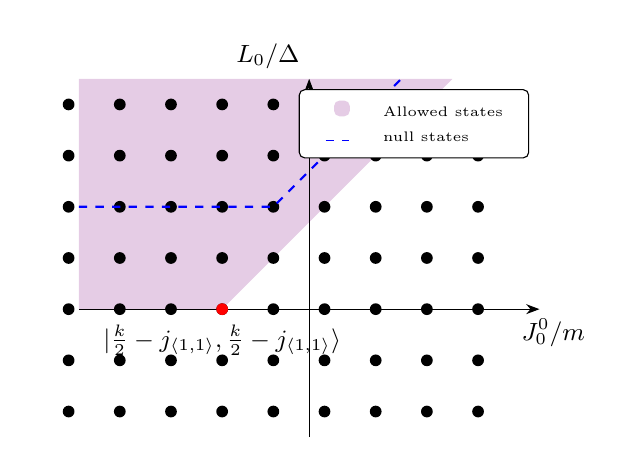
\begin{tikzpicture}[scale=0.65, font=\small]
            \def\xmin{-4.5} \def\xmax{4.5} \def\ymin{-2.5} \def\ymax{4.5}
            \clip (\xmin-1, \ymin) rectangle (\xmax+1, \ymax+1);

            \fill[violet!20] (\xmin, 0) -- (-1.7, 0) -- (\ymax-1.7, \ymax) -- (\xmin, \ymax) -- cycle;
            
            \draw[-{Stealth[]}] (\xmin, 0) -- (\xmax, 0) node[anchor=north west, xshift=-10pt] {$J_0^0/m$};
            \draw[-{Stealth[]}] (0, \ymin) -- (0, \ymax) node[anchor=south east] {$L_0/\Delta$};
            \foreach \x in {-4,...,4} {\foreach \y in {-2,...,4} {\node[dot] at (\x-0.7,\y) {};}}       

            \draw[blue, dashed, thick] (\xmin, 2) -- (-0.7, 2) -- (\ymax-2.7, \ymax) ;
            
            \node[dot, red, label=below:{$|\frac{k}{2}-j_{\vev{1,1}}, \frac{k}{2} - j_{\vev{1,1}} \rangle$}] at (-1.7, 0) {};

            \node[draw, fill=white, rounded corners=2pt, align=left, anchor=north east, font=\tiny] at (\xmax-0.2, \ymax-0.2) {
                \begin{tabular}{rl}\tikz\fill[violet!20](0,0)rectangle(0.2,0.2);&Allowed states\\\tikz\draw[blue,dashed](0,0.1)--(0.3,0.1);&null states\\\end{tabular}};
        \end{tikzpicture}
        \caption{$\widehat{\mathcal{D}}^{-1 - j_{2,1}, -}$}
        \label{fig:D 21_-1}
    \end{subfigure}

    \vspace{1cm}

        \begin{subfigure}[b]{0.48\textwidth}
        \centering
        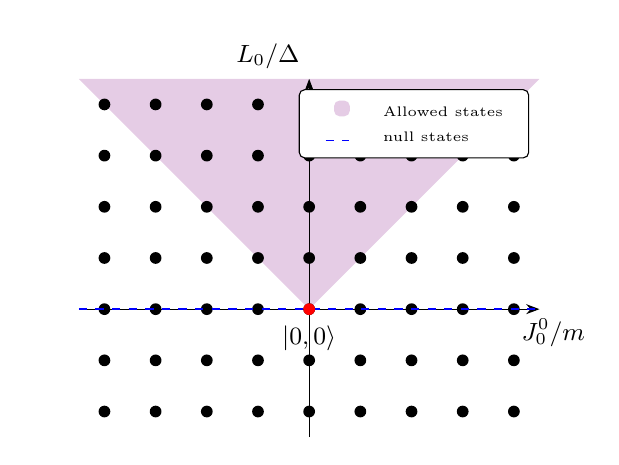
\begin{tikzpicture}[scale=0.65, font=\small]
            \def\xmin{-4.5} \def\xmax{4.5} \def\ymin{-2.5} \def\ymax{4.5}
            \clip (\xmin-1, \ymin) rectangle (\xmax+1, \ymax+1);

            \fill[violet!20] (\xmin, \ymax) -- (0, 0) -- (\xmax, \ymax) -- cycle;

            \draw[-{Stealth[]}] (\xmin, 0) -- (\xmax, 0) node[anchor=north west, xshift=-10pt] {$J_0^0/m$};
            \draw[-{Stealth[]}] (0, \ymin) -- (0, \ymax) node[anchor=south east] {$L_0/\Delta$};
            \foreach \x in {-4,...,4} {\foreach \y in {-2,...,4} {\node[dot] at (\x,\y) {};}}

            \draw[blue, dashed, thick] (\xmin, 0) -- (\xmax, 0) ;
            
            \node[dot, red, label=below:{$|0, 0 \rangle$}] at (0, 0) {};
                                    
            \node[draw, fill=white, rounded corners=2pt, align=left, anchor=north east, font=\tiny] at (\xmax-0.2, \ymax-0.2) {
                \begin{tabular}{rl}\tikz\fill[violet!20](0,0)rectangle(0.2,0.2);&Allowed states\\\tikz\draw[blue,dashed](0,0.1)--(0.3,0.1);&null states\\\end{tabular}};
        \end{tikzpicture}
        \caption{$\widehat{\mathcal{E}}^{0}$}
        \label{fig:E 1_0}
    \end{subfigure}
    \hfill
%fourth picture at down-right corner
    \begin{subfigure}[b]{0.48\textwidth}
        \centering
        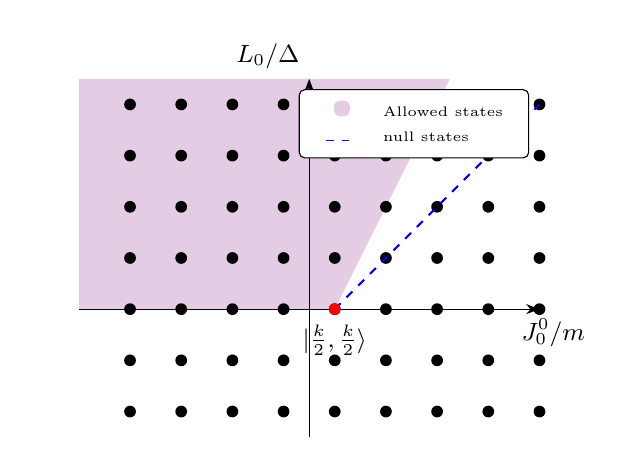
\begin{tikzpicture}[scale=0.65, font=\small]
            \def\xmin{-4.5} \def\xmax{4.5} \def\ymin{-2.5} \def\ymax{4.5}
            \clip (\xmin-1, \ymin) rectangle (\xmax+1, \ymax+1);

            \fill[violet!20] (\xmin, 0) -- (0.5, 0) -- (\ymax/2+0.5, \ymax) -- (\xmin, \ymax) -- cycle;
            
            \draw[-{Stealth[]}] (\xmin, 0) -- (\xmax, 0) node[anchor=north west, xshift=-10pt] {$J_0^0/m$};
            \draw[-{Stealth[]}] (0, \ymin) -- (0, \ymax) node[anchor=south east] {$L_0/\Delta$};
            \foreach \x in {-4,...,4} {\foreach \y in {-2,...,4} {\node[dot] at (\x+0.5,\y) {};}}       

            \draw[blue, dashed, thick] (0.5, 0) -- (\xmax, \xmax-0.5) ;
            
            \node[dot, red, label=below:{$|\frac{k}{2}, \frac{k}{2} \rangle$}] at (0.5, 0) {};
            
            \node[draw, fill=white, rounded corners=2pt, align=left, anchor=north east, font=\tiny] at (\xmax-0.2, \ymax-0.2) {
                \begin{tabular}{rl}\tikz\fill[violet!20](0,0)rectangle(0.2,0.2);&Allowed states\\\tikz\draw[blue,dashed](0,0.1)--(0.3,0.1);&null states\\\end{tabular}};
        \end{tikzpicture}
        \caption{$\widehat{\mathcal{D}}^{-1-j_{\vev{1,1}}, -}$}
        \label{fig:E 1_-1}
    \end{subfigure}

    \caption{Spectra of degenerate representations}
    \label{fig:degrep}
\end{figure}

\newpage

\section{Fusion rules}
In CFT, fusion rules form the algebra of primary fields, dictating how they combine. We could determine the fusion rules from the 
OPE 
\begin{equation}
    \phi^{j_{1},\omega_{1}}(z_{1}) \phi^{j_{2},\omega_{2}}(z_{2}) \sim \sum_{j_{3},\omega_{3}}
    \vev{\phi^{j_{1},\omega_{1}}(z_{1}) \phi^{j_{2},\omega_{2}}(z_{2}) \left(\phi^{j_{3},\omega_{3}}(z_{3}) \right)^{*}} \phi^{j_{3},\omega_{3}}(z_{3}).
\end{equation}
The fusion $\widehat{\mathcal{R}}^{j_{1},\omega_{1}} \widehat{\mathcal{R}}^{j_{2},\omega_{2}} \ni \widehat{\mathcal{R}}^{j_{3},\omega_{3}}$
is allowed only if the 3-point function 
$\vev{\phi^{j_{1},\omega_{1}}(z_{1}) \phi^{j_{2},\omega_{2}}(z_{2}) \left(\phi^{j_{3},\omega_{3}}(z_{3}) \right)^{*}}$ is non-zero.

On the other hand, the null vector equations give constraint on the 3-point functions involving degenerate fields. In this chapter, we 
will use the null vector equations to determine fusion rules of some degenerate representations.

\subsection{Fusion rules with the spectral flowed vacuum representation}
We conjecture that the spectral flow commutes with fusion, which has been proved in some specific cases \cite{Gaberdiel:2001ny}, 
\begin{equation}
    \rho_{\omega_{1}} \left(\widehat{\mathcal{R}}^{j_{1}}\right) \times \rho_{\omega_{2}} \left(\widehat{\mathcal{R}}^{j_{2}}\right) = \rho_{\omega_{1} + \omega_{2}} \left(\widehat{\mathcal{R}}^{j_{1}}\times \widehat{\mathcal{R}}^{j_{2}} \right). \label{SpecFus}
\end{equation}
In order to prove this conjecture, one could consider the spectral flowed vacuum representation. Since the fusion between any 
representation $\widehat{\mathcal{R}}^{j}$ with the vacuum representation $\widehat{\mathcal{E}}^{0}$ should give 
$\widehat{\mathcal{R}}^{j}$ back: 
\begin{equation}
    \widehat{\mathcal{E}}^{0} \times \widehat{\mathcal{R}}^{j} = \widehat{\mathcal{R}}^{j}.
\end{equation}
Hence from our conjecture \eqref{SpecFus}, we find 
\begin{equation}
    \rho_{\omega} \left( \widehat{\mathcal{E}}^{0} \right) \times \widehat{\mathcal{R}}^{j} = \rho_{\omega} \left( \widehat{\mathcal{R}}^{j} \right).
\end{equation}

Let's prove this fusion rule for $\omega = \pm 1$ by using the null vector appears in the spectral flowed vacuum representation, namely 
$J^{-}_{-1}\ket{\frac{k}{2}, - \frac{k}{2}}=0$. The corresponding null vector equation in the $m$-basis is 
\begin{equation}
    \vev{J^{-}_{-1} \phi^{\frac{k}{2}}_{-\frac{k}{2}, \bar{m}_{1}}(z_{1}, \bar{z_{1}}) 
     \phi^{j_{2}}_{m_{2},\bar{m}_{2}}(z_{2},\bar{z_{2}}) \phi^{j_{3},-1}_{m_{3},\bar{m}_{3}}(z_{3},\bar{z_{3}}) } = 0.
\end{equation}
By using the local Ward identity, we obtain
\begin{equation}
    \begin{aligned}
        0 = &\vev{J^{-}_{-1} \phi^{-j_{\vev{1,1}}-1}_{j_{\vev{1,1}}+1}(z_{1}) \phi^{j_{2}}_{m_{2}}(z_{2}) \phi^{j_{3}}_{m_{3}}(z_{3})} \\
        =& -\frac{1}{z_{21}} \vev{ \phi^{-j_{\vev{1,1}}-1}_{j_{\vev{1,1}}+1}(z_{1}) J^{-}_{0} \phi^{j_{2}}_{m_{2}}(z_{2}) \phi^{j_{3}}_{m_{3}}(z_{3})} \\
        &- \frac{1}{z_{31}} \vev{ \phi^{-j_{\vev{1,1}}-1}_{j_{\vev{1,1}}+1}(z_{1}) \phi^{j_{2}}_{m_{2}}(z_{2}) \rho_{-1}\left(J^{-}_{-1}\right) \phi^{j_{3}}_{m_{3}}(z_{3})} 
        + \frac{1}{(z_{31})^{2}} \vev{ \phi^{-j_{\vev{1,1}}-1}_{j_{\vev{1,1}}+1}(z_{1}) \phi^{j_{2}}_{m_{2}}(z_{2}) \rho_{-1}\left(J^{-}_{0}\right) \phi^{j_{3}}_{m_{3}}(z_{3})}.
    \end{aligned}
\end{equation}
Substituting the global Ward identity \eqref{GlobalWard} to the above null vector equation, 
we find the null vector equation is simplified to 
\begin{equation}
    (\frac{1}{z_{21}}- \frac{1}{z_{31}}) \vev{ \phi^{-j_{\vev{1,1}}-1}_{j_{\vev{1,1}}+1}(z_{1}) J^{-}_{0} \phi^{j_{2}}_{m_{2}}(z_{2}) \phi^{j_{3}}_{m_{3}}(z_{3})} - 
    \frac{1}{(z_{31})^{2}} \vev{ \phi^{-j_{\vev{1,1}}-1}_{j_{\vev{1,1}}+1}(z_{1}) \phi^{j_{2}}_{m_{2}}(z_{2}) \rho_{-1}\left(J^{-}_{0}\right) \phi^{j_{3}}_{m_{3}}(z_{3})} = 0.
\end{equation}
Substitute the spectral flow violating 3-point function \eqref{3pointfunc_m-1}, 
since $\Delta^{j_{3},-1}_{m_{3}-1} = \Delta^{j_{3},-1}_{m_{3}} - 1$, we find the $z$-dependence of the two terms is exactly the same. 
The equation is simplified to 
\begin{equation}
            (j_{2}+m_{2}) (j_{2}+1 - m_{2}) - (j_{3}+m_{3})(j_{3}+1-m_{3}) = 0. \label{nullvectoreq0m}
\end{equation}
The conservation of $m$ gives 
\begin{equation}
    j_{\vev{1,1}} +1 + m_{2} - 1 + m_{3} + \frac{k}{2} = 0
\end{equation}
Substitute the exact expression of $j_{\vev{1,1}} = -\frac{k+2}{2}$, we find 
\begin{equation}
    m_{3} + m_{2} -1 = 0.
\end{equation}
substitute it into \eqref{nullvectoreq0m}, we find 
\begin{equation}
    j_{2}(j_{2} + 1) = j_{3}(j_{3}+1).
\end{equation}
It shows that the quadratic Casimir operator for $j_{2}$ and $j_{3}$ is the same, which means they correspond to the same representation.
Hence we obtain the following fusion rule.
\begin{equation}
    \rho_{1} \left(\widehat{\mathcal{E}}^{0}\right) \times \widehat{\mathcal{R}}^{j} = \rho_{1} \left( \widehat{\mathcal{R}}^{j} \right).
\end{equation}
In addition, this fusion rule proves our conjecture \eqref{SpecFus} in the simplest cases: 
\begin{equation}
    \begin{aligned}
        \rho_{\pm 1} \left( \widehat{\mathcal{R}}^{j_{1}} \right) \times \widehat{\mathcal{R}}^{j_{2}} & = 
        \left(\rho_{\pm 1} \left(\widehat{\mathcal{E}}^{0}\right) \times \widehat{\mathcal{R}}^{j_{1}} \right) \times \widehat{\mathcal{R}}^{j_{2}} \\
        &= \rho_{\pm 1} \left(\widehat{\mathcal{E}}^{0}\right) \times \Big(\widehat{\mathcal{R}}^{j_{1}} \times \widehat{\mathcal{R}}^{j_{2}} \Big) \\
        &= \rho_{\pm 1} \left( \widehat{\mathcal{R}}^{j_{1}} \times \widehat{\mathcal{R}}^{j_{2}} \right).
    \end{aligned}
\end{equation}

\subsection{Fusion rules with level 1 degenerate representations}

\subsubsection*{Spectral flow preserving case}

The vanishing of the null vector $\hat{N}^{c}_{1,1} \phi^{\vev{1,1}}_{x,\bar{x}} = 0$ gives the following equation:
\begin{equation}
    \vev{\hat{N}^{c}_{1,1} \phi^{\vev{1,1}}_{x_{1},\bar{x_{1}}}(z_{1},\bar{z_{1}}) \phi^{j_{2}}_{x_{2},\bar{x_{2}}}(z_{2},\bar{z_{2}})
     \phi^{j_{3}}_{x_{3},\bar{x_{3}}}(z_{3}, \bar{z_{3}})} = 0.
\end{equation}
We substitute the local Ward identity \eqref{LocalWard}, and get the following differential 
equation:
\begin{equation}
    \begin{aligned}
        0 = &\sum_{s=2,3} \frac{1}{z_{s1}}
        \Big\{ K_{a b} D_{x_s}\left(t^a\right) D_{x_1}\left(t^c\right) D_{x_1}\left(t^b\right)+ j_{\vev{1,1}} f_{a b}^c D_{x_s}\left(t^a\right) D_{x_1}\left(t^b\right) \\
        & - 2 j_{\vev{1,1}}^2 D_{x_s}\left(t^c\right) \Big\}
        \vev{\phi^{1,1}_{x_{1}}(z_{1}) \phi^{j_{2}}_{x_{2}}(z_{2}) \phi^{j_{3}}_{x_{3}}(z_{3})}  = 0.
    \end{aligned}
     \label{nullvectoreqx}
\end{equation}
We use the conformal symmetry to send $z_{1}, z_{2}, z_{3} \rightarrow 0,1,\infty$, where only the term proportional to $\frac{1}{z_{21}}$ 
survives. Then the null vector equation corresponding to $c=-$ is simplified to 
\begin{equation}
    \begin{aligned}
        &\left\{ x_{12}^2 \partial_{1}^{2} \partial_{2} + 2 j_{2} x_{12} \partial_{1}^{2} + 2 (1-2j_{\vev{1,1}})x_{12} \partial_{1}\partial_{2} \right. \\
        &\left. + 2 (1-2j_{\vev{1,1}})j_{2} \partial_{1} -2j_{\vev{1,1}}(1-2j_{\vev{1,1}}) \partial_{2} \right\} D^{\mathbf{1}} \left[\begin{array}{ccc}
    j_{1} & j_2 & j_3 \\
    x_1 & x_2 & x_3
    \end{array} \right] = 0 ,
    \end{aligned}
\end{equation}
where $\partial_{i} = \frac{\partial}{\partial x_{i}}$. By substituting the 3-point function in the $x$-basis \eqref{3pointfuncx}, we get the following condition on the spins: 
\begin{equation}
    \left( j_{\vev{1,1}}^{2} - (j_{2}-j_{3})^{2} \right)(1+j_{\vev{1,1}}+j_{2}+j_{3}) = 0.
\end{equation}
The solution to this equation is $j_{3} = j_{2} \pm j_{\vev{1,1}}, -j_{2} - 1 + j_{\vev{1,1}}$. Since the above equation 
is symmetric for $j_{2}$ and $j_{3}$, the other term in \eqref{nullvectoreqx} proportional to $\frac{1}{z_{31}}$ should give 
the same condition. 

Therefore we determine the following fusion rule:
\begin{equation}
    \widehat{\mathcal{R}}^{1,1} \times \widehat{\mathcal{R}}^{j} \supset \widehat{\mathcal{R}}^{j+j_{\vev{1,1}}} + \widehat{\mathcal{R}}^{j-j_{\vev{1,1}}}.
\end{equation}
In addition, the other two null vector equations of $c = 0,+$ can be deduced from \eqref{CRJN}. Hence all three null vector equations give the 
same fusion rule. 

\subsubsection*{Spectral flow violating case}
Now let's consider the spectral violating case, namely:
\begin{equation}
    \vev{\hat{N}^{c}_{1,1} \phi^{\vev{1,1}}(z_{1},\bar{z_{1}}) \phi^{j_{2}}(z_{2},\bar{z_{2}})
     \phi^{j_{3},\pm 1}(z_{3}, \bar{z_{3}})} = 0.
\end{equation}
We will solve the above null vector equation in the $m$-basis.

The null vector at level 1 \eqref{nullvectorm} gives the following equation:
\begin{equation}
    \begin{aligned}
            0 = & \vev{J^{+}_{-1} \phi^{\vev{1,1}}_{m_{1}-1,\bar{m_{1}}}(z_{1},\bar{z_{1}}) 
        \phi^{j_{2}}_{m_{2},\bar{m_{2}}}(z_{2},\bar{z_{2}}) \phi^{j_{3},-1}_{m_{3},\bar{m_{3}}}(z_{3},\bar{z_{3}})} \\
        &+ 2\vev{J^{0}_{-1} \phi^{\vev{1,1}}_{m_{1},\bar{m_{1}}}(z_{1},\bar{z}_{1}) 
        \phi^{j_{2}}_{m_{2},\bar{m_{2}}}(z_{2},\bar{z_{2}}) \phi^{j_{3},-1}_{m_{3},\bar{m_{3}}}(z_{3},\bar{z_{3}})} \\
        &- \vev{J^{-}_{-1} \phi^{\vev{1,1}}_{m_{1}+1,\bar{m_{1}}}(z_{1},\bar{z_{1}}) \phi^{j_{2}}_{m_{2},\bar{m_{2}}}(z_{2},\bar{z_{2}}) 
        \phi^{j_{3},-1}_{m_{3},\bar{m_{3}}}(z_{3},\bar{z_{3}})} .
    \end{aligned}
\end{equation}
Substituting the local Ward identity, the equation is equivalent to 
\begin{equation}
    \begin{aligned}
        0 = & \quad \frac{1}{z_{21}}\vev{ \phi^{\vev{1,1}}_{m_{1}-1,\bar{m_{1}}}(z_{1},\bar{z_{1}}) J^{+}_{0}
        \phi^{j_{2}}_{m_{2},\bar{m_{2}}}(z_{2},\bar{z_{2}}) \phi^{j_{3},-1}_{m_{3},\bar{m_{3}}}(z_{3},\bar{z_{3}})}  
        +\frac{2}{z_{21}}\vev{
        \phi^{\vev{1,1}}_{m_{1},\bar{m_{1}}}(z_{1},\bar{z}_{1}) J^{0}_{0}
        \phi^{j_{2}}_{m_{2},\bar{m_{2}}}(z_{2},\bar{z_{2}}) \phi^{j_{3},-1}_{m_{3},\bar{m_{3}}}(z_{3},\bar{z_{3}})} \\
        & +\frac{2}{z_{31}}\vev{
         \phi^{\vev{1,1}}_{m_{1},\bar{m_{1}}}(z_{1},\bar{z}_{1}) 
        \phi^{j_{2}}_{m_{2},\bar{m_{2}}}(z_{2},\bar{z_{2}}) J^{0}_{0} \phi^{j_{3},-1}_{m_{3},\bar{m_{3}}}(z_{3},\bar{z_{3}})} 
        -\frac{1}{z_{21}}\vev{
        \phi^{\vev{1,1}}_{m_{1}+1,\bar{m_{1}}}(z_{1},\bar{z_{1}}) J^{-}_{0} \phi^{j_{2}}_{m_{2},\bar{m_{2}}}(z_{2},\bar{z_{2}}) 
        \phi^{j_{3},-1}_{m_{3},\bar{m_{3}}}(z_{3},\bar{z_{3}})}\\ 
        & - \frac{1}{z_{31}}\vev{
        \phi^{\vev{1,1}}_{m_{1}+1,\bar{m_{1}}}(z_{1},\bar{z_{1}}) \phi^{j_{2}}_{m_{2},\bar{m_{2}}}(z_{2},\bar{z_{2}}) 
        \rho_{-1}\left(J^{-}_{-1}\right) \phi^{j_{3},-1}_{m_{3},\bar{m_{3}}}(z_{3},\bar{z_{3}})} \\
        & +\frac{1}{(z_{31})^{2}}\vev{
        J^{-}_{-1} \phi^{\vev{1,1}}_{m_{1}+1,\bar{m_{1}}}(z_{1},\bar{z_{1}}) \phi^{j_{2}}_{m_{2},\bar{m_{2}}}(z_{2},\bar{z_{2}}) 
        \rho_{-1}\left(J^{-}_{0}\right) \phi^{j_{3},-1}_{m_{3},\bar{m_{3}}}(z_{3},\bar{z_{3}})} .
    \end{aligned}
\end{equation}
Substituting the 3-point function, again we find the $z$-dependence cancels and the equation is reduced to 
\begin{equation}
    (-j_{\vev{1,1}}-1+m_{1}+2m_{2})(-j_{\vev{1,1}}+m_{1}) - (m_{3}-m_{2})((1-m_{3}-m_{2})) + j_{2}(j_{2}+1) - j_{3}(j_{3}+1) = 0. \label{nullvectoreqm}
\end{equation}
The conservation of $m$ now gives 
\begin{equation}
    m_{1} + m_{2} + m_{3} + \frac{k}{2} = 0.
\end{equation}
Since we have $j_{\vev{1,1}} = -\frac{k+2}{2}$, we can substitute $\frac{k}{2}$ by $-j_{\vev{1,1}} - 1$. We find 
\begin{equation}
    j_{\vev{1,1}} - m_{1} = m_{2} + m_{3} - 1 . 
\end{equation}
The null vector equation \eqref{nullvectoreqm} is simplified to: 
\begin{equation}
    j_{2}(j_{2}+1) - j_{3}(j_{3}+1) = 0.
\end{equation}
Again we find the quadratic Casimir opeartor for $j_{2}$ and $j_{3}$ is the same, which gives the following fusion rule:
\begin{equation}
    \widehat{\mathcal{R}}^{\vev{1,1}} \times \widehat{\mathcal{R}}^{j} \supset \rho_{1} \left( \widehat{\mathcal{R}}^{j} \right).
\end{equation}
The fusion rule should be symmetric for $\rho_{\pm 1}$, hence we should also have 
\begin{equation}
    \widehat{\mathcal{R}}^{\vev{1,1}} \times \widehat{\mathcal{R}}^{j} \supset \rho_{-1} \left( \widehat{\mathcal{R}}^{j} \right).
\end{equation}

In conclusion, we conjecture the fusion rule between a degenerate representation and a generic affine highest-weight representation to be: 
\begin{equation}
    \boxed{
        \widehat{\mathcal{R}}^{\vev{1,1}} \times \widehat{\mathcal{R}}^{j} = \widehat{\mathcal{R}}^{j+j_{\vev{1,1}}} \oplus \widehat{\mathcal{R}}^{j-j_{\vev{1,1}}}
    \oplus \rho_{1} \left( \widehat{\mathcal{R}}^{j} \right) \oplus \rho_{-1} \left( \widehat{\mathcal{R}}^{j} \right).
    } \label{mainresult}
\end{equation}

\newpage

\section{Conclusion and outlook}
In this thesis, we investigated the fusion rules between degenerate representations and affine highest weight representations. 
We determined that the fusion with spectral flowed vacuum representation gives the spectral flowed representation, thereby proving our conjecture 
that the spectral flow commutes with fusion in the simplest cases. We also gave the fusion rule between level 1 degenerate representations 
with affine highest representations as \eqref{mainresult}, 
which implies that the fusion between level 1 degenerate representations may give spectral flowed representations.

In the future, one possible generalization of our results is to extend the fusion rules with spectral flowed vacuum representations 
to generic $\omega \in \mathbb{Z}$. This could potentially be proven by induction. One can also use the fusion rule with level 1 
degenerate representations to test the conjectured fusion rules between affine highest weight representations given in 
\cite{Maldacena:2001km}.

\section*{Acknowledgement}
I would like to express my deepest gratitude to my master’s advisor, Professor Sylvain Ribault, for his unwavering support and insightful 
advice on my research. I am especially thankful for his invaluable mentorship in shaping my approach to research, 
from formulating questions to rigorously pursuing solutions. 

I am also very grateful to the Institut de Physique Théorique (IPhT) at CEA Saclay for the invaluable internship opportunity that 
greatly enriched this research. Finally, I wish to thank both École Polytechnique and ETH Zürich for providing an excellent academic 
environment and for their support throughout my studies.

\printbibliography[heading=bibintoc]
\end{document}